\chapter{SW implementering og test }

\section{Implementering}
Softwaren i blodtryksmåleren er opbygget omkring 3-lags modellen. 

\begin{figure}[H]
	\centering
	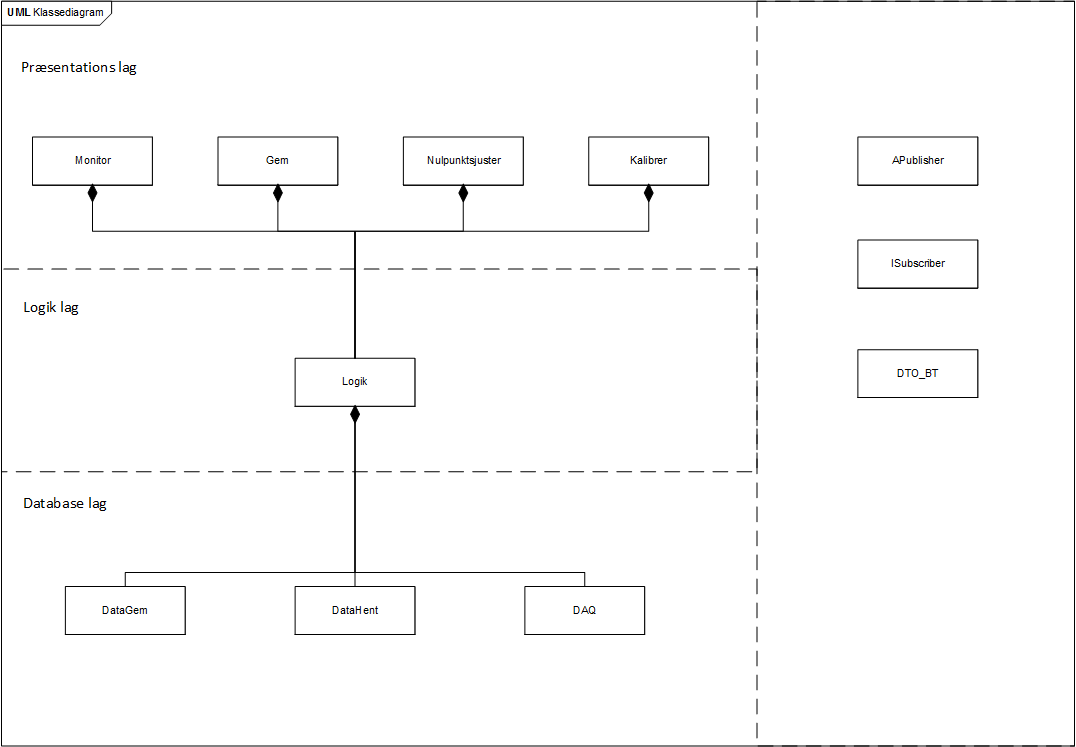
\includegraphics[width=1\textwidth]{Figurer/3lagsmodel_software}
	\caption{UML kompositions klassediagram}
\end{figure}

\begin{figure}[H]
	\centering
	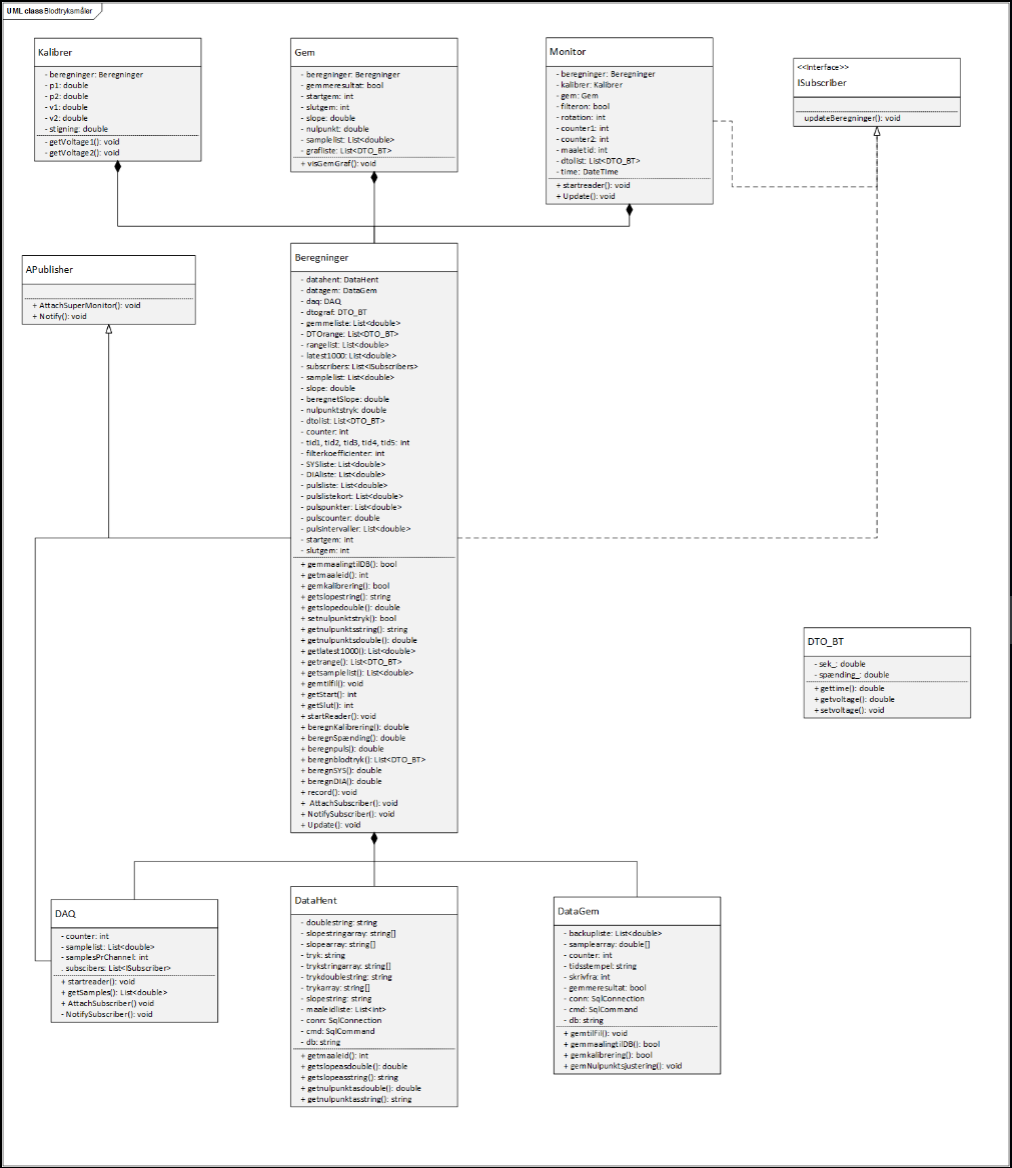
\includegraphics[width=1\textwidth]{Figurer/classdiagram}
	\caption{Klassediagram}
\end{figure}

\subsection{Datalag}
Datalaget kommunikerer med DAQ, database og computers HDD. 

\subsubsection{DAQ}
Herunder er en klasse, DAQ, hovedsageligt med software fra National Instruments, der kan udveksle data med den fysiske DAQ 6009. Denne kan betragtes som af typen ”black box”. Dette betyder at undertegnede ikke har et begreb om den interne mekanisme i klassen. Som udgangspunkt ved vi at funktionen af klassen er at levere data omkring de målinger der foretages i den fysiske DAQ.\\
De styrbare parametre i denne klasse er bl.a.: Sampling frekvens og måleområde. 

\subsubsection{Datahent}
Klassen henter data fra database og lokale tekstfiler. Fra databasen indhentes data om tidligere målingers nummerering således at de målinger der skal gemmes i fremtiden kan blive nummereret korrekt.\\
De lokale tekstfiler indeholder data omkring tidligere kalibreringer og nulpunktsjusteringer.

\subsubsection{DataGem}
Klassen gemmer data, på database, og lokale tekstfiler.

\subsection{Logik lag}

\subsubsection{Beregninger}
Beregninger er hovedsageligt et lag hvor logiske beregninger foretages.\\
Herunder beregnes ting som systolisk og diastolisk blodtryk og puls. Beregninger i forbindelse med kalibrering og nulpunktsjustering foregår også her. Ydermere forbinder logik laget data laget med form laget. Dette tillader at metoder fra datalaget kan anvendes fra form laget.

\subsection{Præsentations lag}
\begin{figure}[H]
	\centering
	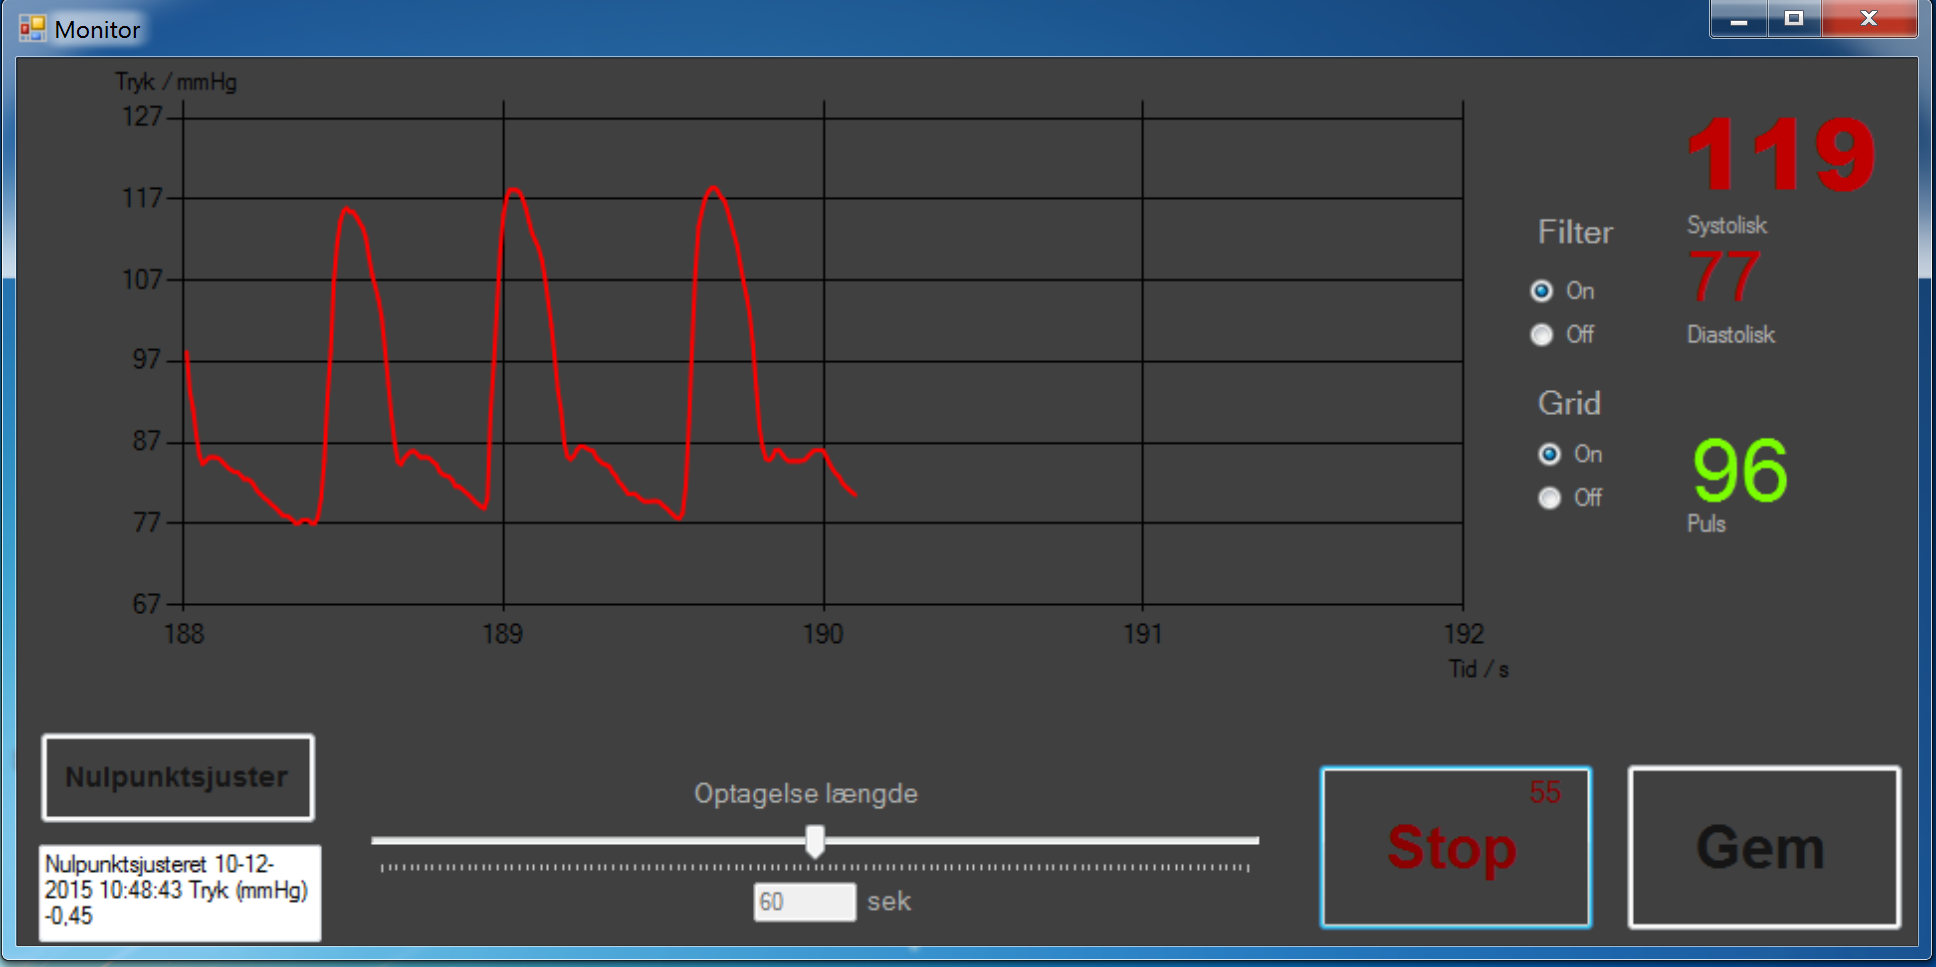
\includegraphics[width=1\textwidth]{Figurer/Monitor_vindue_Recording}
	\caption{Monitor med igangsat måling}
\end{figure}

\subsubsection{Monitor}
Monitorlaget er forskerens generelle visuelle interaktionslag med systemet. Heri observeres udskrevne blodtrykssignaler over 4-sekunders intervaller. Værdierne puls, systolisk og diastolisk blodtryk udskrives også her. Designet er inspireret fra i forvejen eksisterende blodtryks monitoreringssystemer. \\
Der er mulighed for at vælge en længde af optagelse af måling, op påbegyndelse/stoppe med en ”Rec” knap. Herefter kan gem vinduet åbnes hvor den optagne sekvens kan gemmes. Der er en knap til udførelse af nulpunktsjustering. Den kørende måling kan vises med et filter, eller uden med 2 radio butons. Y- og X-akse kan påsættes med 2 radio buttons. 

\subsubsection{Gem}
Vinduet udskriver den optagne sekvens i et vindue der visuelt ligner monitor vinduet. Der er to tekstbokse, hvor en kommentar og et navn, for den ansvarlige af målingen, kan indtastes.
\begin{figure}[H]
	\centering
	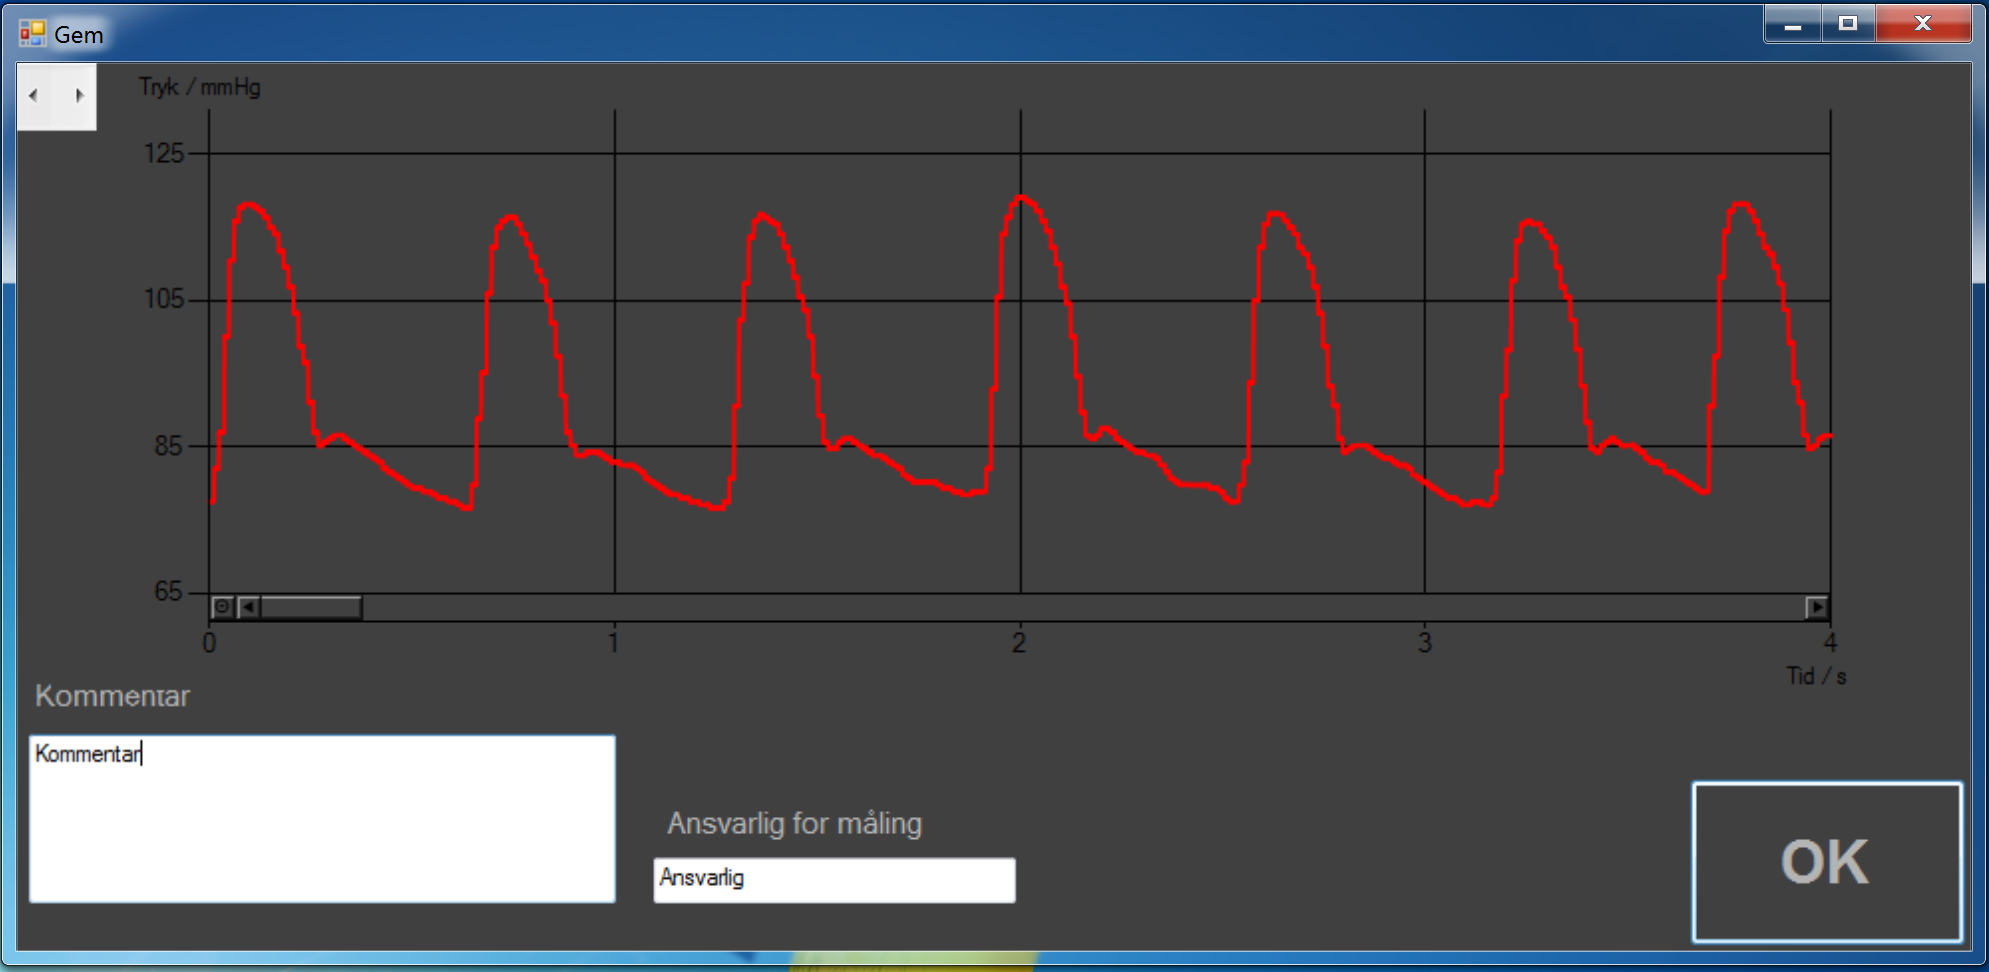
\includegraphics[width=1\textwidth]{Figurer/Gem}
	\caption{Gem vindue, med 10 sekunders måling}
\end{figure}

\subsubsection{Kalibrer}
Vinduet indeholder to tekstbokse til indtastning af tryk og tekstbokse til dertilhørende spænding. Spændingerne kan måles automatisk ved tryk på knapperne ”mål”.
Kalibreringskonstanten kan udregnes med knappen ”Beregn”, og gemmes og anvendes ved tryk på ”OK” knappen.

\subsection{DTO}
DTO er et namespace det indeholder data transfer object (DTO). Alle den andre lag ”kender” dette lag, og kan oprette instanser af klassen DTO.\\
Denne klasse har attributterne tid og spænding. Formålet med denne klasse er at overføre sampleværdier fra DAQ i et format der har en korrekt tidsværdi, samt et tryk (blodtryk) korrigeret for nulpunktstryk samt kalibrering.
\begin{figure}[H]
	\centering
	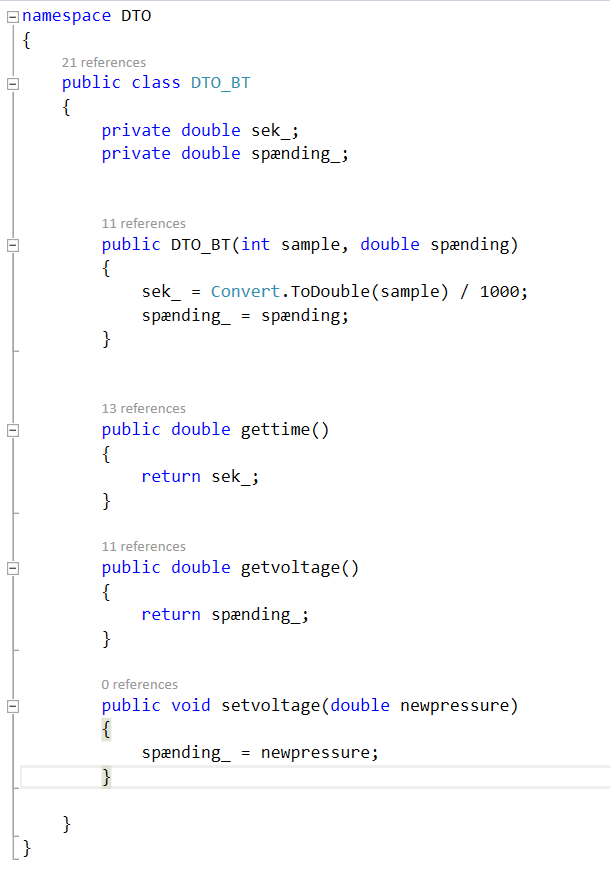
\includegraphics[width=0.5\textwidth]{Figurer/DTO_kode}
	\caption{DTO klassen med metoder}
\end{figure}

\subsubsection{Publisher/subscriber pattern}
Data ”strømmen” fra DAQ klassen, er styrende for alle de andre klasser, bl.a. udskrivning af blodtrykket i monitor vinduet. Den fysiske DAQ måler i med 1000 Hz og returnerer data til DAQ klassen med 50 ms intervaller. Dette måleinterval indeholder 50 sampleværdier. Disse data sendes videre til beregninger klassen, og fra beregninger klassen til monitor klassen vha. Publisher/Subscriber mønstret. Når data befinder sig i monitor klassen kan der laver logiske beregninger og manipulation på data i beregninger klassen.
Forholdet imellem klasserne er således; DAQ klassen og beregninger klassen har et publisher/subscriber forhold, og  beregninger og monitor har et publisher/subscriber forhold. \\
Hierakiet fremgår af figurerne herunder.
\begin{figure}[H]
	\centering
	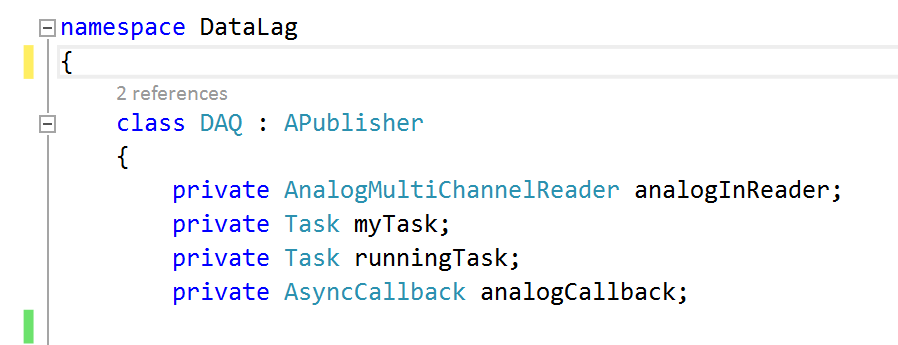
\includegraphics[width=0.5\textwidth]{Figurer/DAQ_pub}
	\caption{DAQ klassens arvehieraki}
\end{figure}

\begin{figure}[H]
	\centering
	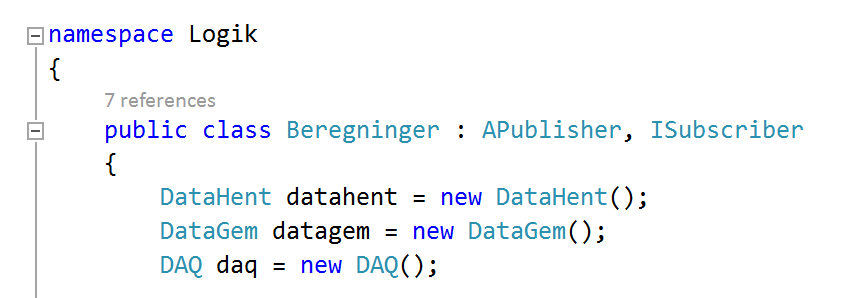
\includegraphics[width=0.5\textwidth]{Figurer/Beregninger_subpub}
	\caption{Beregninger klassens arvehieraki}
\end{figure}

\begin{figure}[H]
	\centering
	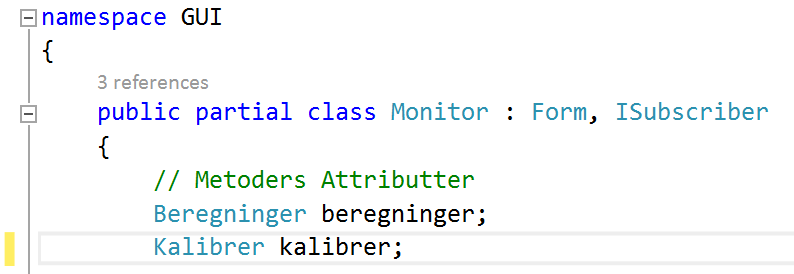
\includegraphics[width=0.5\textwidth]{Figurer/Monitor_sub}
	\caption{Monitor klassens arvehieraki}
\end{figure}


\subsection{Metodebeskrivelser}
Metoden der beregner puls, har to logiske grene til udregning af pulsen. Den første (til venstre i diagram) regner pulsen når der er mellem 3000 og 10000 samples til rådighed, altså når den fysiske DAQ har målt imellem 3 og 10 sekunder.\\
Metodikken består i at lokalisere toppunkter i signalet, for at udregne det gennemsnitlige interval herimellem. Herudfra kan pulsen estimeres. \\
En for-løkke bruges til at evaluere alle sampleværdier i forhold til de før liggende og efterfølgende samples. Hvis værdien på den pågældende sample har større værdi end den før liggende og efterfølgende, gemmes tidspunktet for dette sample i en liste.\\ 
For at sikre at ”toppunktet” ikke er et mindre toppunkt, fra fx støj eller højfrekvent signalindhold, evalueres der kun for hver 50'ende værdier, og tidspunktet gemmes kun hvis værdien ligger 0,1 V over gennemsnittet af alle sampleværdier der evalueres. Ud fra gennemsnitsintervallet imellem toppunkterne beregnes pulsen.
\\
\\
Den anden logiske gren regner pulsen når der er over 10000 samples til rådighed, altså efter den fysiske DAQ har målt i over 10 sekunder.\\ 
Metodikken er den samme som ovenfor, men i stedet for at gemme et tidspunkt for toppunktet, tælles en counter op. Når antallet af toppunkter for 10 sekunder er fundet, kan pulsen beregnes.

\begin{figure}[H]
	\centering
	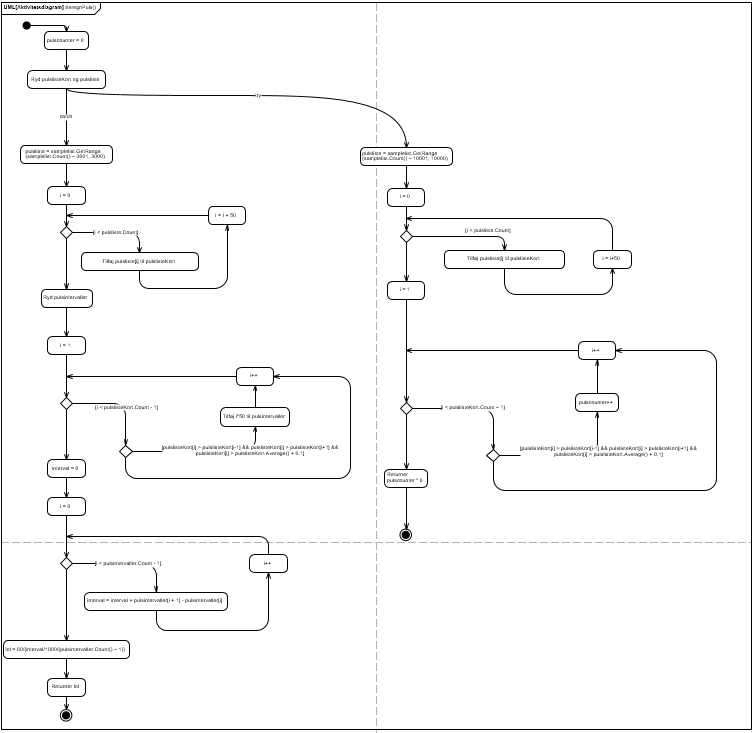
\includegraphics[width=1\textwidth]{Figurer/aktivitetsdiagram_beregnPuls}
	\caption{Aktivitetsdiagram over beregnpuls}
\end{figure}


\subsection{Sekvensdiagrammer}
Sekvensdiagrammerne beskriver kommunikationen imellem software klasserne der er involveret i de respektive Use Cases.\\

\subsubsection{UC1}
Forsker trykker på knappen "Beregn" anmoder kalibrerings klassen om metoden 'beregn' i klassen Beregninger. Den udregnede kalibreringskonstant returneres.\\
Forsker trykker på knappen "OK" og metoden 'gemkalibrering' afvikles i klassen beregninger. Herfra afvikles metoden gemkalibrering i Datagem klassen. Datagem returnerer en bool der beskriver om gemningen var succesfuld.
\begin{figure}[H]
	\centering
	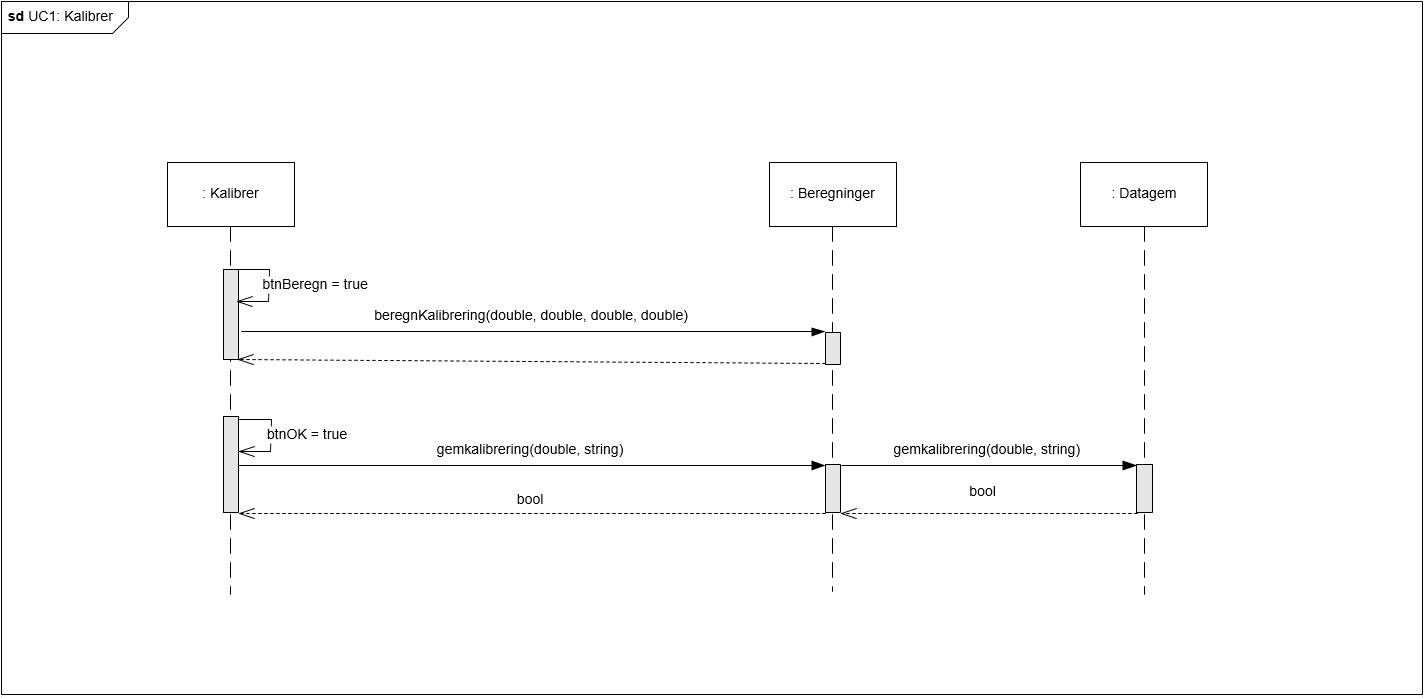
\includegraphics[width=1\textwidth]{Figurer/UC1_SD_SW}
	\caption{Sekvensdiagram for UC1}
\end{figure}

\subsubsection{UC2}
Når monitor vinduet åbnes (når programmet starter) afvikles metoden 'startreader' i DAQ. Vha. publisher/subscriber metoden 'NotifySubscriber' returneres rådata til Beregninger og videre til Monitor.\\
Rådata sendes til Beregninger og omregnes til tid og blodtryk vha DTO klassen.
'beregnSYS', 'beregnDIA' og 'beregnPuls' returnerer ligeledes double værdier med systolisk og diastolisk blodtryk samt puls.
\begin{figure}[H]
	\centering
	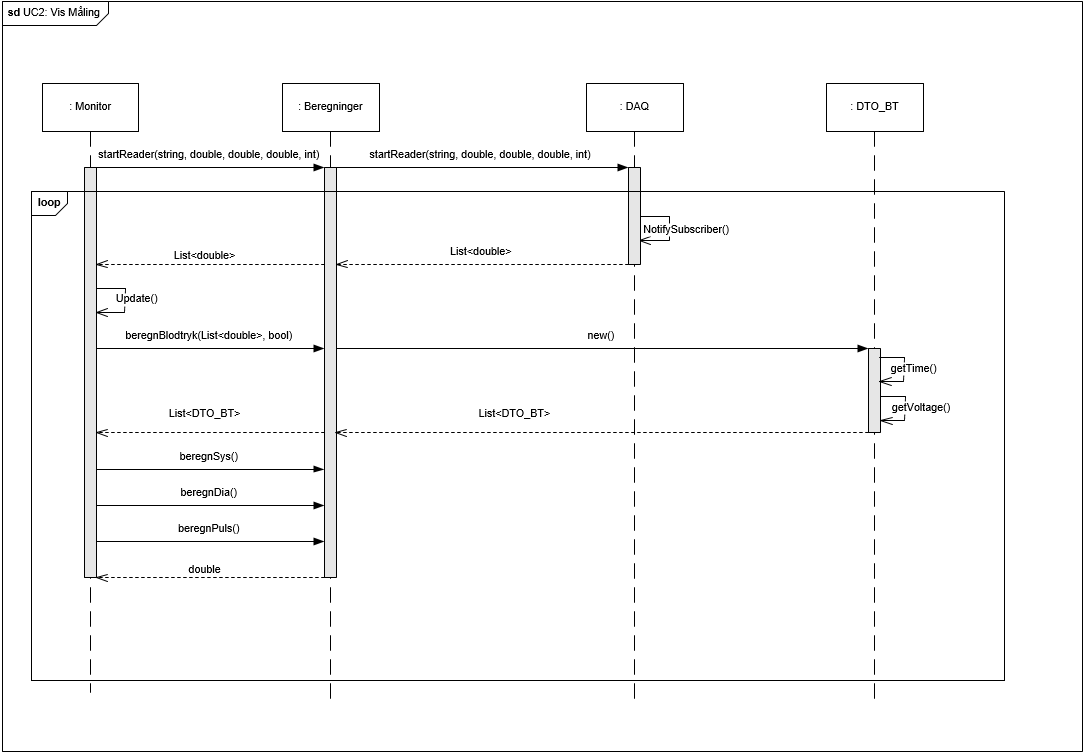
\includegraphics[width=1\textwidth]{Figurer/UC2_SD_SW}
	\caption{Sekvensdiagram for UC2}
\end{figure}

\subsubsection{UC3}
'getNulpunktsstring' returnerer en string der indeholder data om seneste nulpunktsjustering. Denne udskrives på Monitor.\\
Forsker trykker på knappen 'Nulpunktsjuster' og Beregninger udfører en nulpunktsjustering, gemmer data i Datagem, og returnerer en ny string der beskriver seneste (denne) nulpunktsjusterin.

\begin{figure}[H]
	\centering
	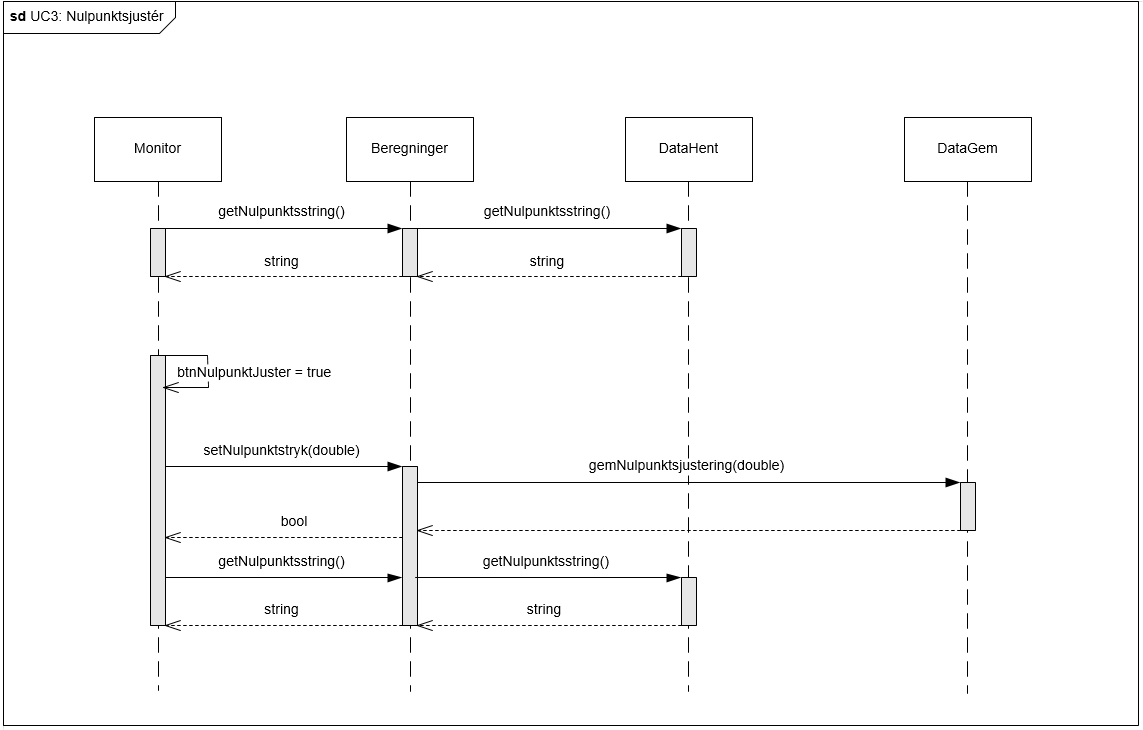
\includegraphics[width=1\textwidth]{Figurer/UC3_SD_SW}
	\caption{Sekvensdiagram for UC3}
\end{figure}
\subsubsection{UC4}
Forsker sætter radibutton til filter til "off".
Bool "filteron" sættes til false, og sendes med metoden der udregner blodtryk' beregnBlodtryk', i beregninger. Den returnerede liste af DTO'er, som udskrives i Monitor, er ufiltrerede.

\begin{figure}[H]
	\centering
	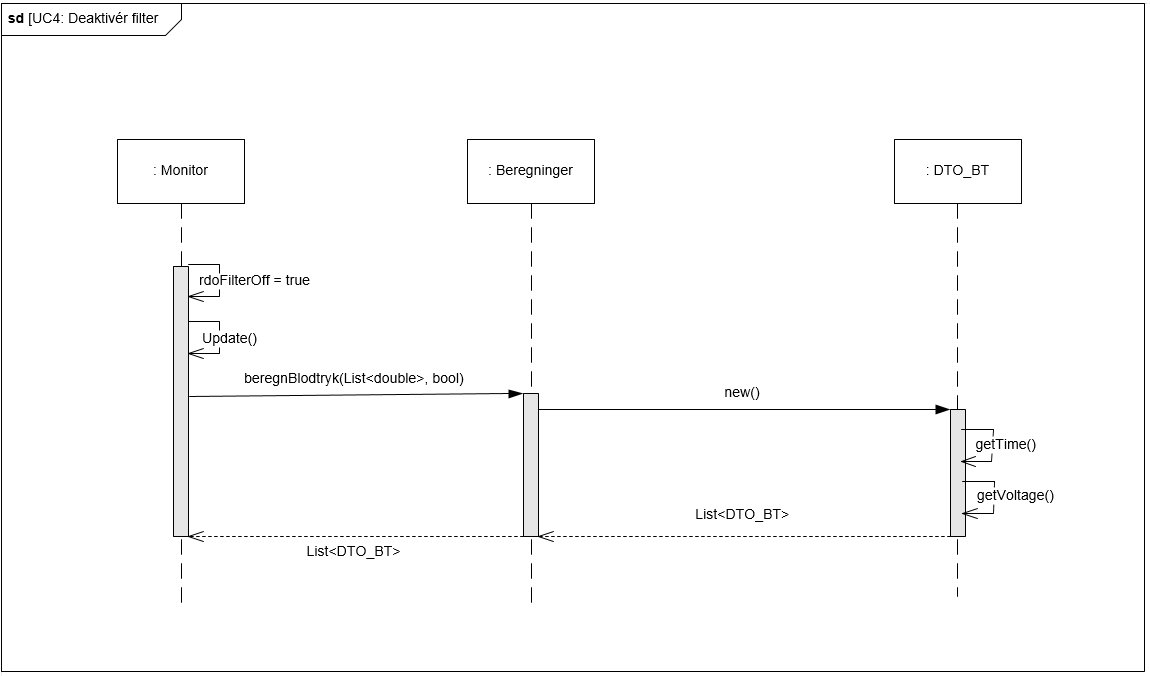
\includegraphics[width=1\textwidth]{Figurer/UC4_SD_SW}
	\caption{Sekvensdiagram for UC4}
\end{figure}

\subsubsection{UC5}
Forsker sætter radibutton til filter til "on".
Bool "filteron" sættes til true, og sendes med metoden der udregner blodtryk 'beregnBlodtryk', i beregninger. Den returnerede liste af DTO'er, som udskrives i Monitor, er filtrerede.

\begin{figure}[H]
	\centering
	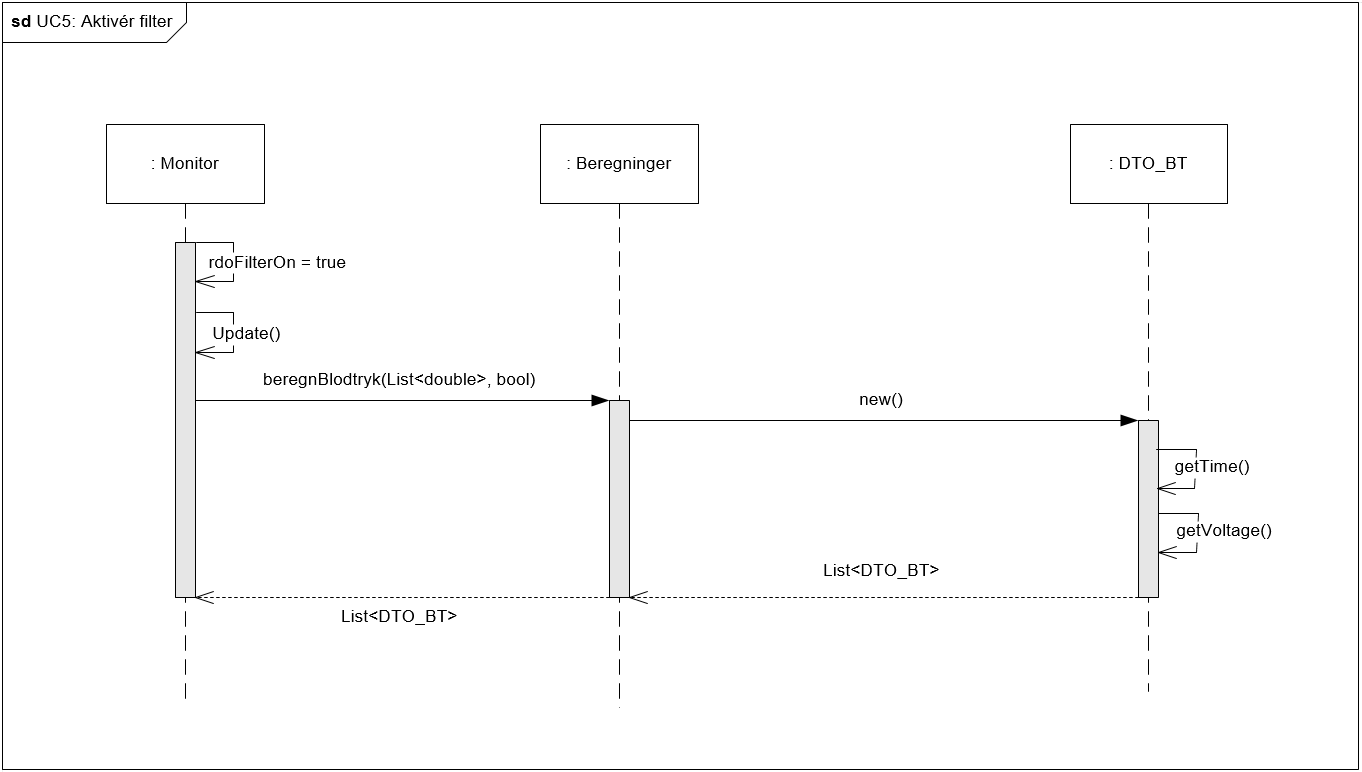
\includegraphics[width=1\textwidth]{Figurer/UC5_SD_SW}
	\caption{Sekvensdiagram for UC5}
\end{figure}

\subsubsection{UC6}
Forsker vælger en optagelseslængde og trykker på "record". Monitor-vinduet sender så en bool til beregninger der startes en optagelse af signalet. Når 

\begin{figure}[H]
	\centering
	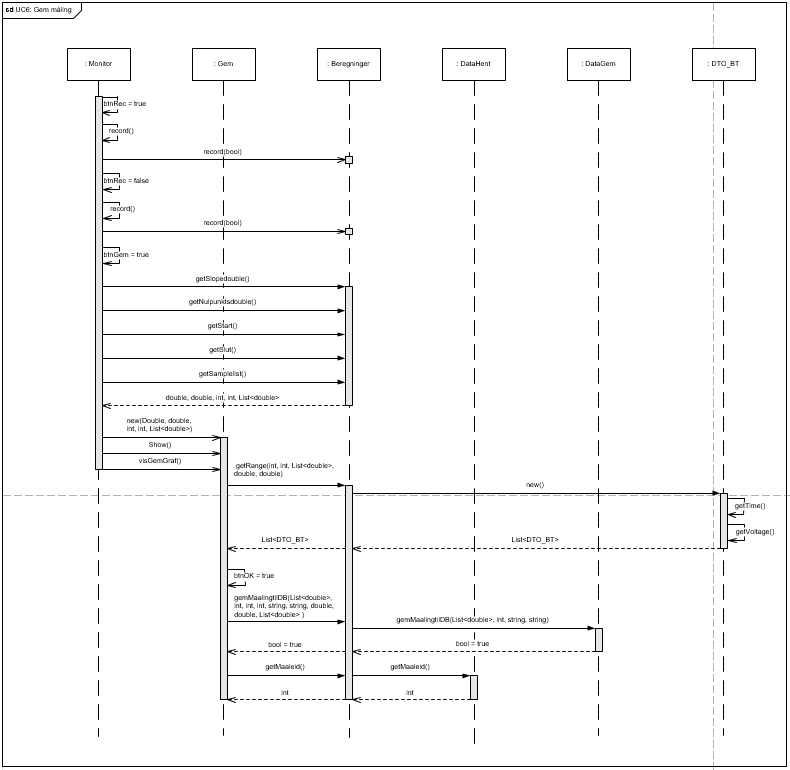
\includegraphics[width=1\textwidth]{Figurer/UC6_SD_SW}
	\caption{Sekvensdiagram for UC6}
\end{figure}

\section{Test}
Til at teste de forskellige metoder i softwaren har benyttes debugging. Debugging gør det muligt at følge compilerens sekventielle udførelse af programmet. Når der udføres handlinger og attributværdier sættes kan dette følges, og sættes op mod de forventede resultater. Såfremt der skulle opstå fejl gør debugging det muligt at fokuserer på enkelte metoder og undersøge, hvor fejlen opstår.
\subsection{Puls}
Til at teste pulsmetoden startes en optagelse fra starten af målingen. Målelængden sættes til 10 sek. Disse parametre sætte i monitor-vinduets constructor.
\begin{figure}[H]
	\centering
	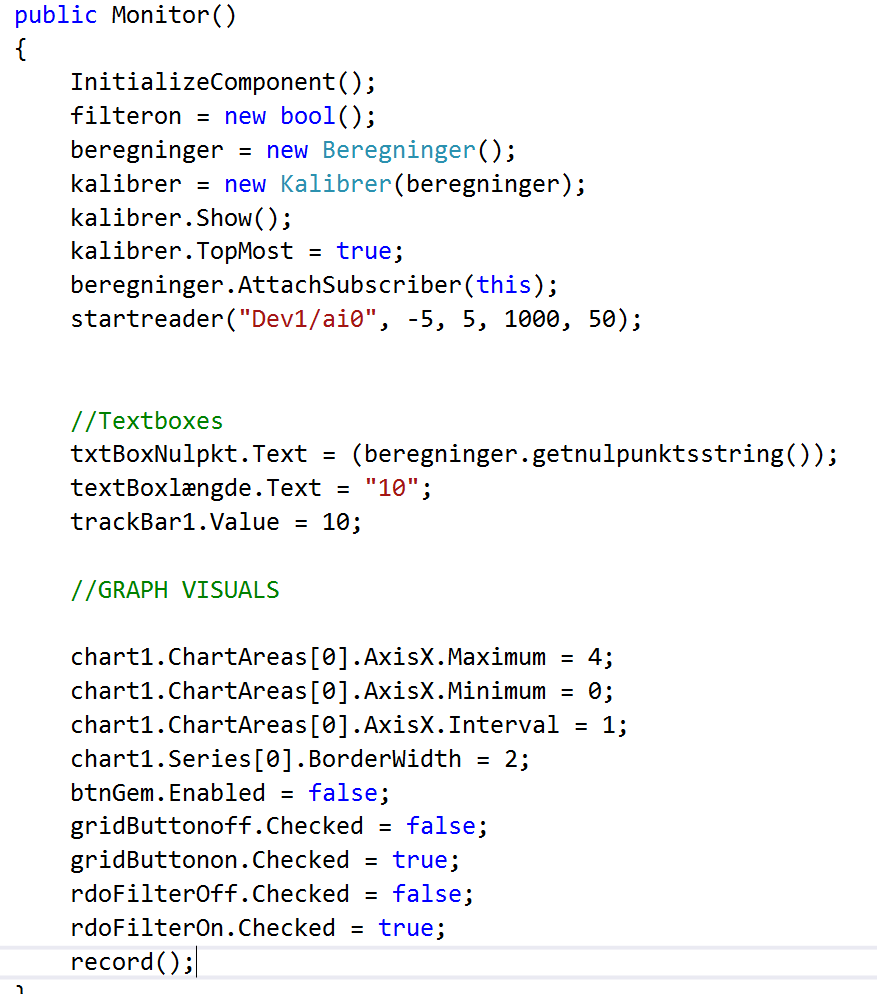
\includegraphics[width=0.5\textwidth]{Figurer/Pulstest_record}
	\caption{Monitor vinduets default constructor ved puls-test}
\end{figure}
Et break point sættes ved metoden der returnerer en puls efter baseret på 10000 samples. Metoden har talt 15 pulsslag.
\begin{figure}[H]
	\centering
	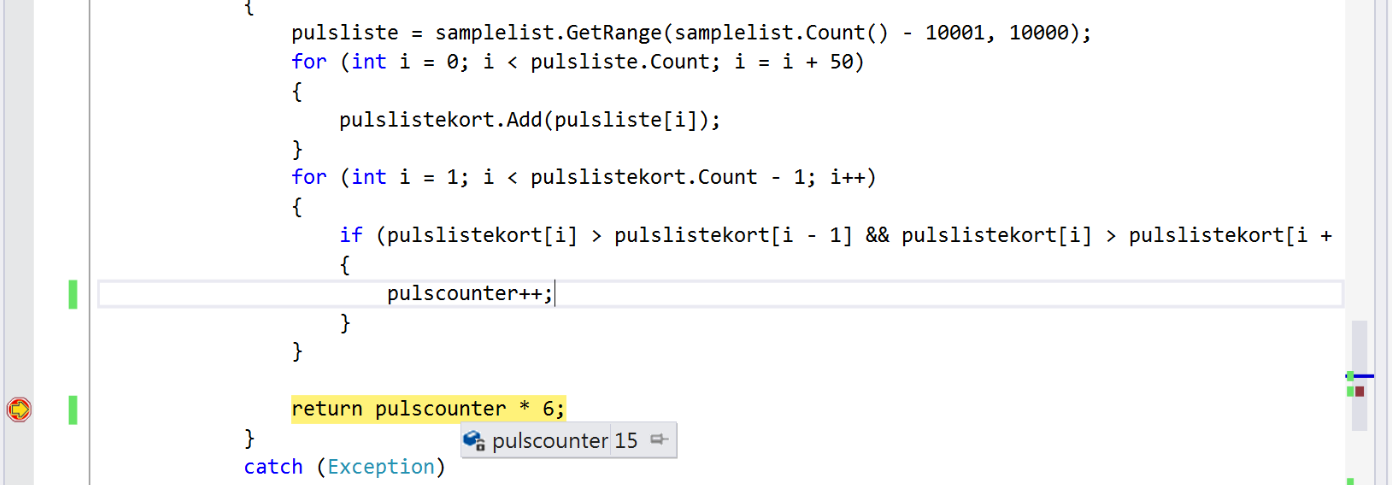
\includegraphics[width=1\textwidth]{Figurer/Pulstest_debug}
	\caption{Puls efter 10 sekunders måling}
\end{figure}
Antallet af pulsslag tællet på gem vinduet for de 10 sekunder. Her er der talt 15 pulsslag. Kun 4 sekunder kan vises ad gangen.
\begin{figure}[H]
	\centering
	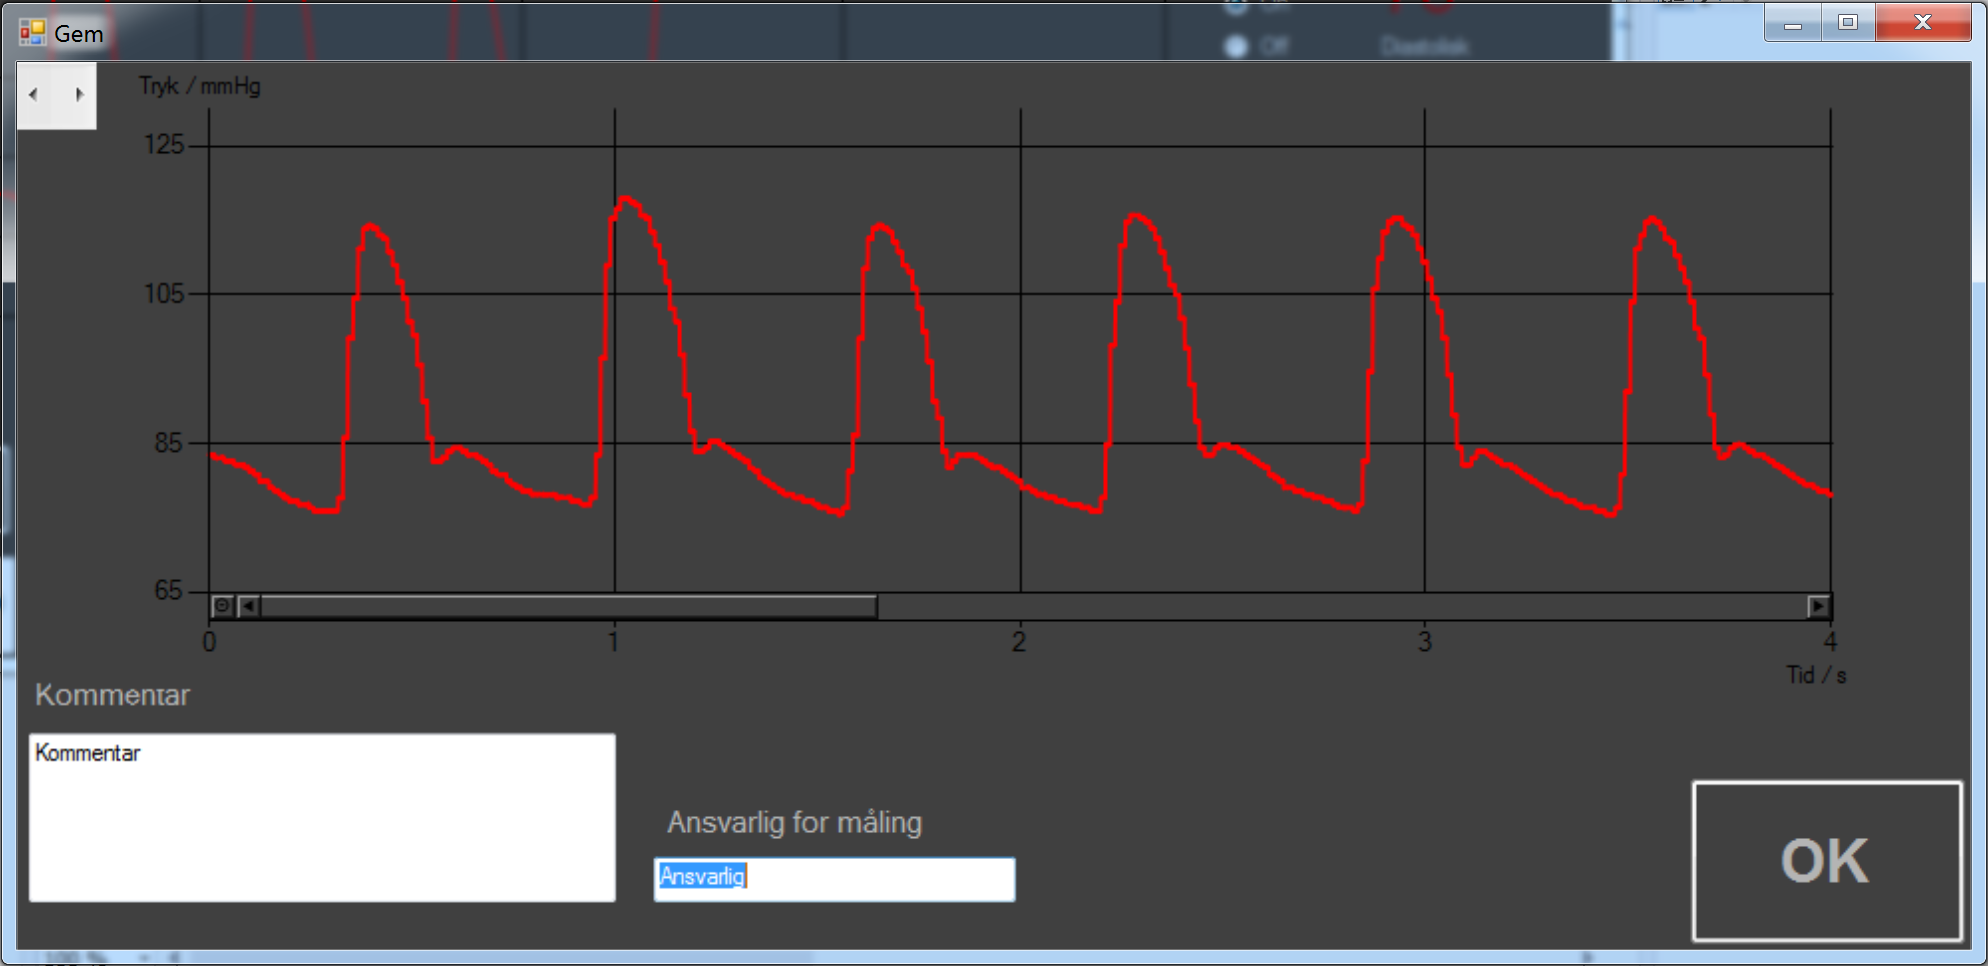
\includegraphics[width=1\textwidth]{Figurer/Pulstest_gemmevindue}
	\caption{Puls efter 10 sekunders måling}
\end{figure}

Det talte antal pulsslag holdes op mod dem der er talt af metoden beregnpuls.

\begin{figure}[H]
	\centering
	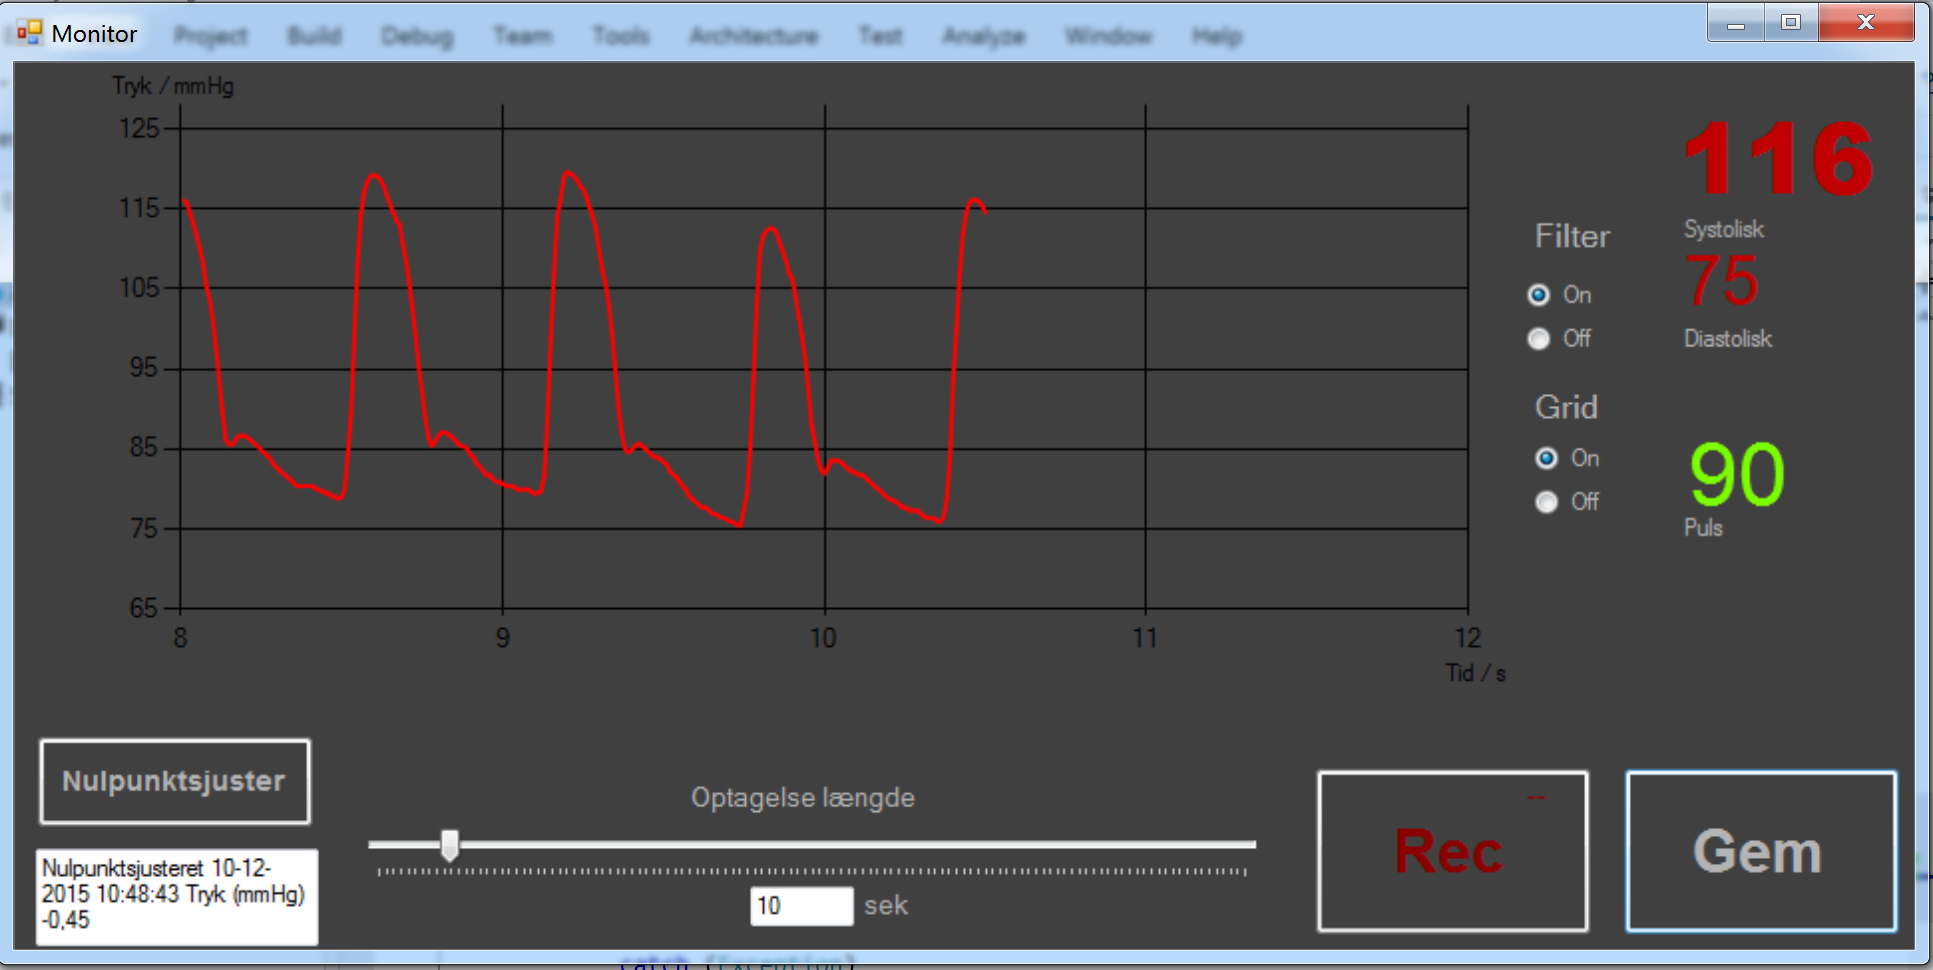
\includegraphics[width=1\textwidth]{Figurer/Pulstest_monitor}
	\caption{Puls efter 10 sekunders måling}
\end{figure}


Den beregnede puls er 90, hvilket stemmer overens med 15 pulsslag på 10 sekunder.Denne test kan bekræfte at metoden fungerer efter hensigten.

\subsection{UC1 Kalibrer}

Forsker indtaster (målte) kalibreringsdata. Kalibreringsdata for seneste kalibreringsdata vises.

\begin{figure}[H]
	\centering
	\includegraphics[width=1\textwidth]{Figurer/Test_Kalibrer_1}
	\caption{Kalibreringsdata indtastet}
\end{figure}

De målte værdier beregnes.

\begin{figure}[H]
	\centering
	\includegraphics[width=1\textwidth]{Figurer/Test_Kalibrer_2}
	\caption{Kalibreringskonstant udregnes}
\end{figure}

Kalibreringskonstanten implementeres ved udskrivning på graf.
\begin{figure}[H]
	\centering
	\includegraphics[width=1\textwidth]{Figurer/Test_Kalibrer_3}
	\caption{Kalibreringsdata anvendes}
\end{figure}
Det kontrolleres at kalibreringsfilen er opdateret
\begin{figure}[H]
	\centering
	\includegraphics[width=1\textwidth]{Figurer/Test_Kalibrer_4}
	\caption{Kalibreringsdata er gemt til fil}
\end{figure}

\subsection{UC2 Vis måling}
Et inputsignal på 1 Hz, 1 V amplitude og 0 V offset bruges til input på den fysiske DAQ. 
\begin{figure}[H]
	\centering
	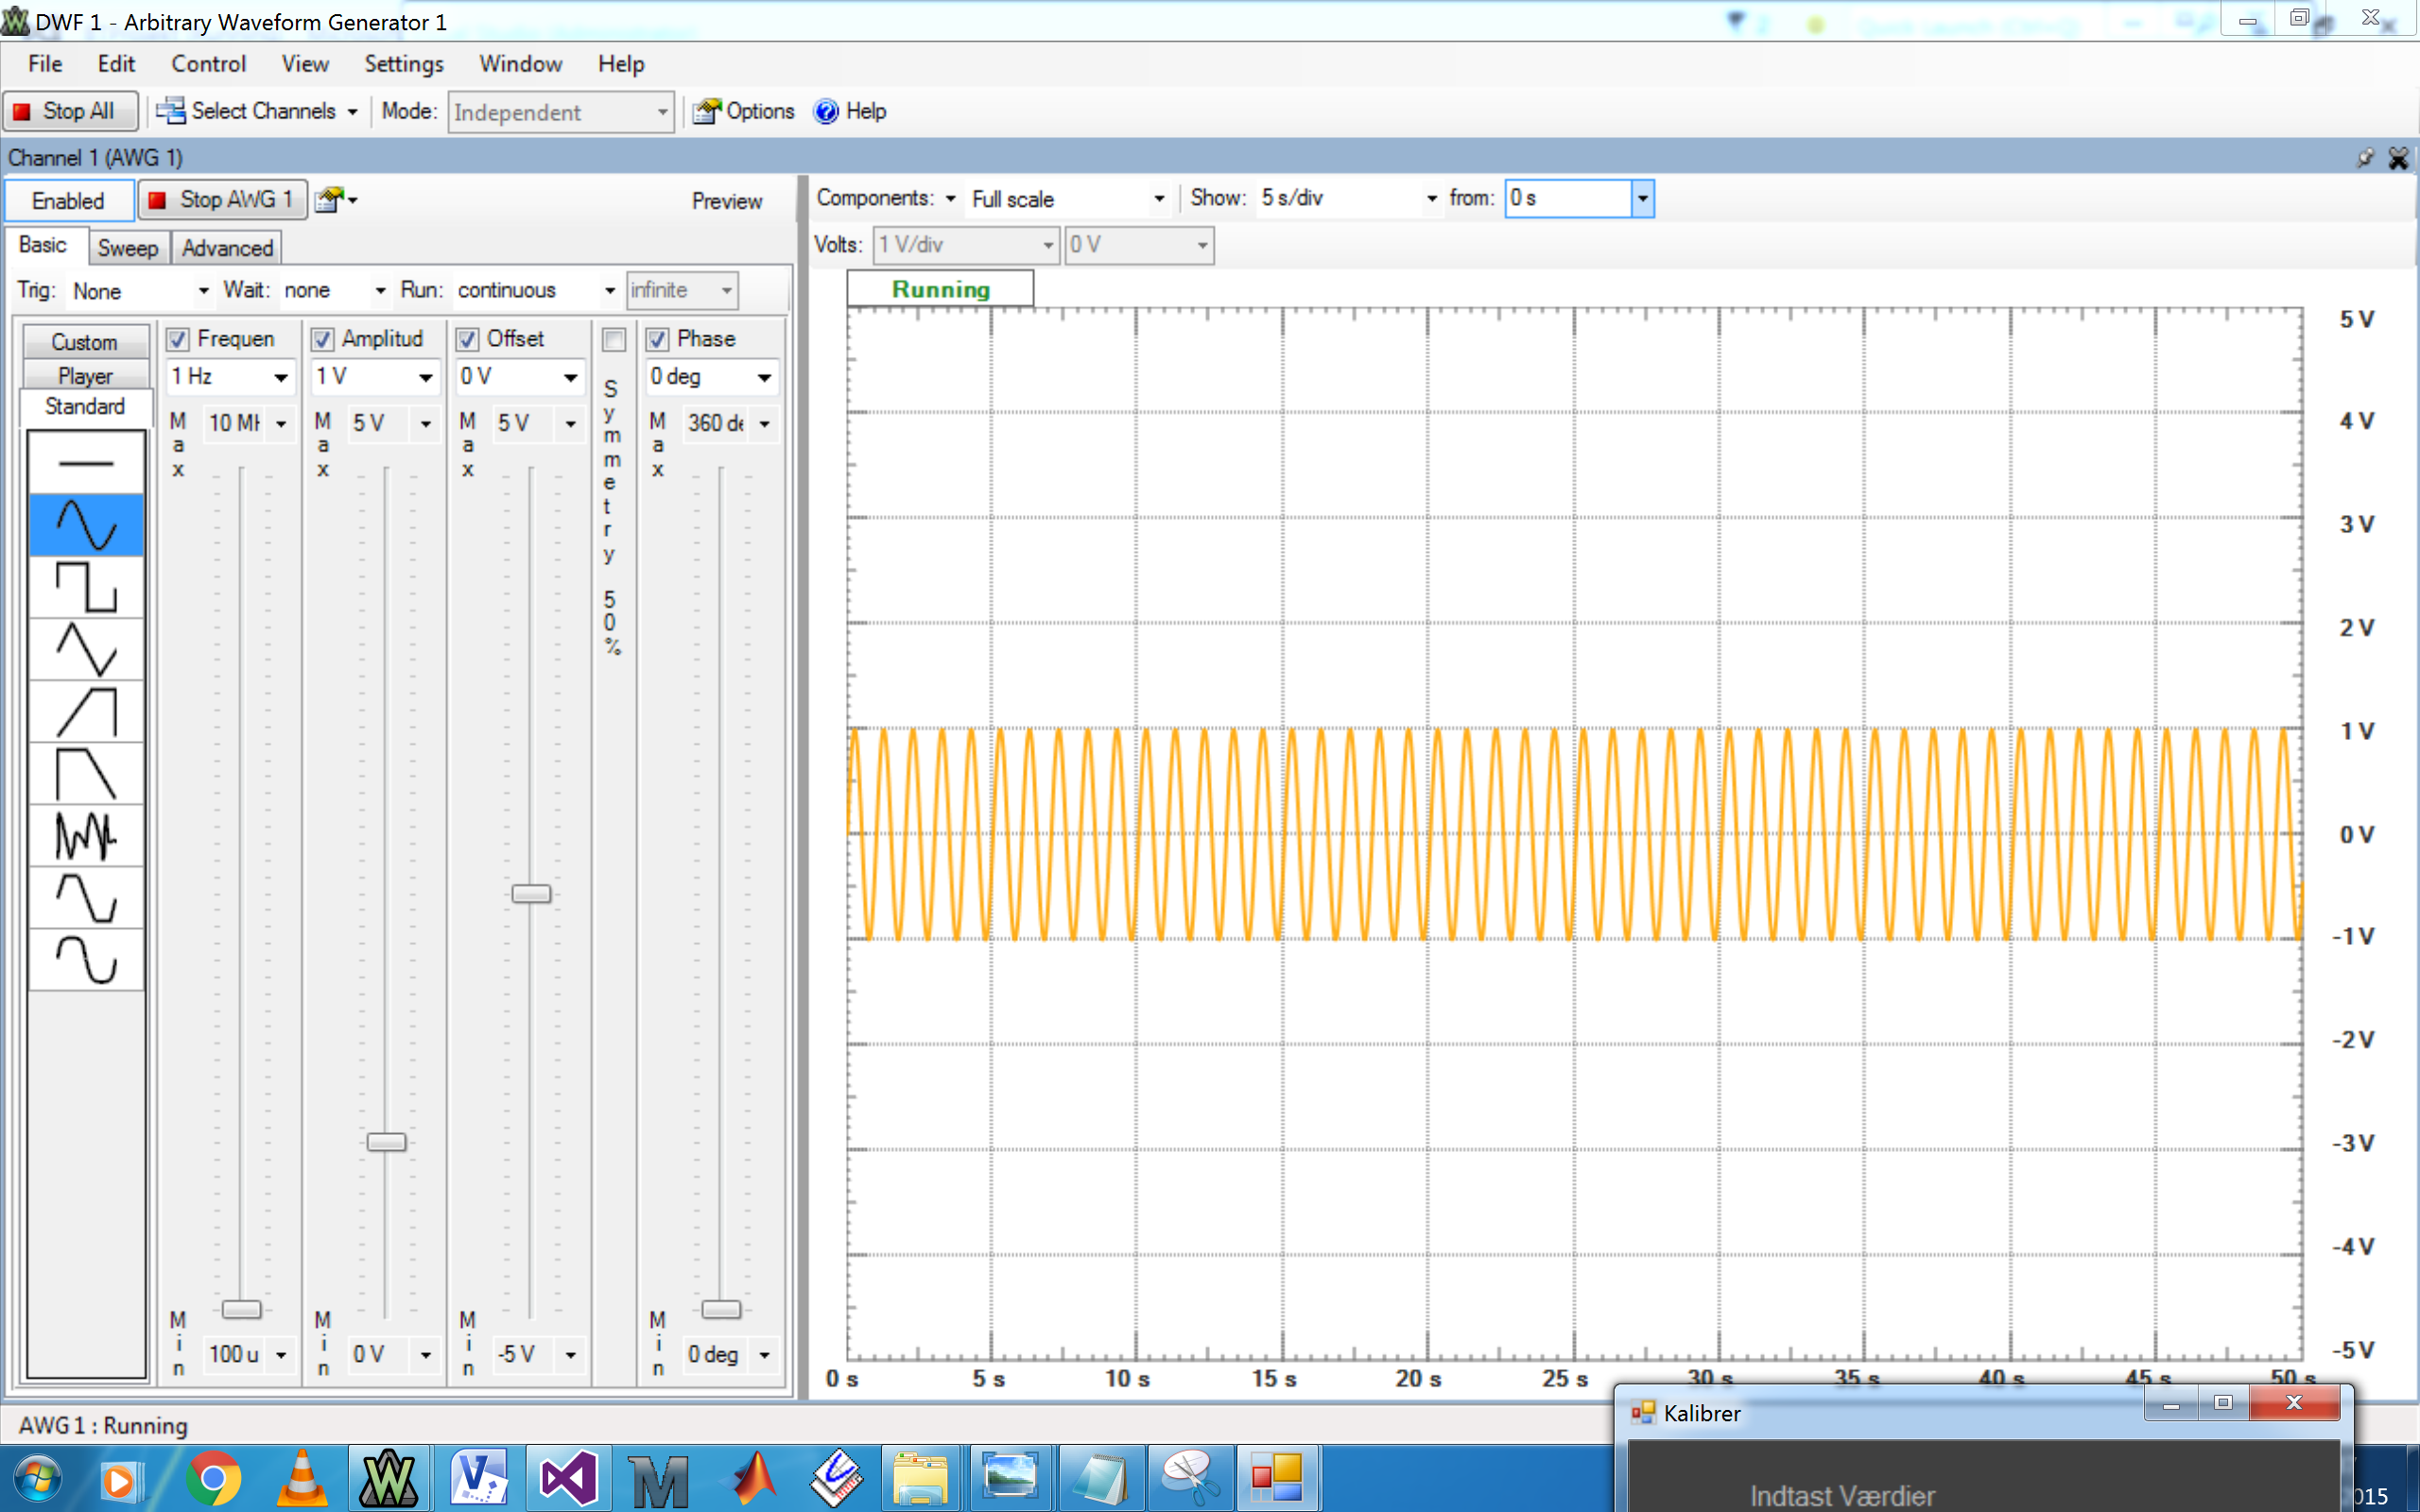
\includegraphics[width=1\textwidth]{Figurer/Test_Vis_1}
	\caption{Inputsignal til DAQ}
\end{figure}

Det ses at kalibreringskonstanten (mmHg/V) = 57,9.
Nulpunktsjusteringsværdien er tæt på 0.
Maksværdien på signalet (Systole) skal være 58 mmHg.
Minimumsværdien på signalet skal være -58mmHg. 
Pulsen skal være 60 = 1 Hz.

Kalibreringskonstante er 57,9. Det udskrevne "blodtryk" er 57,9 mm Hg.
\begin{figure}[H]
	\centering
	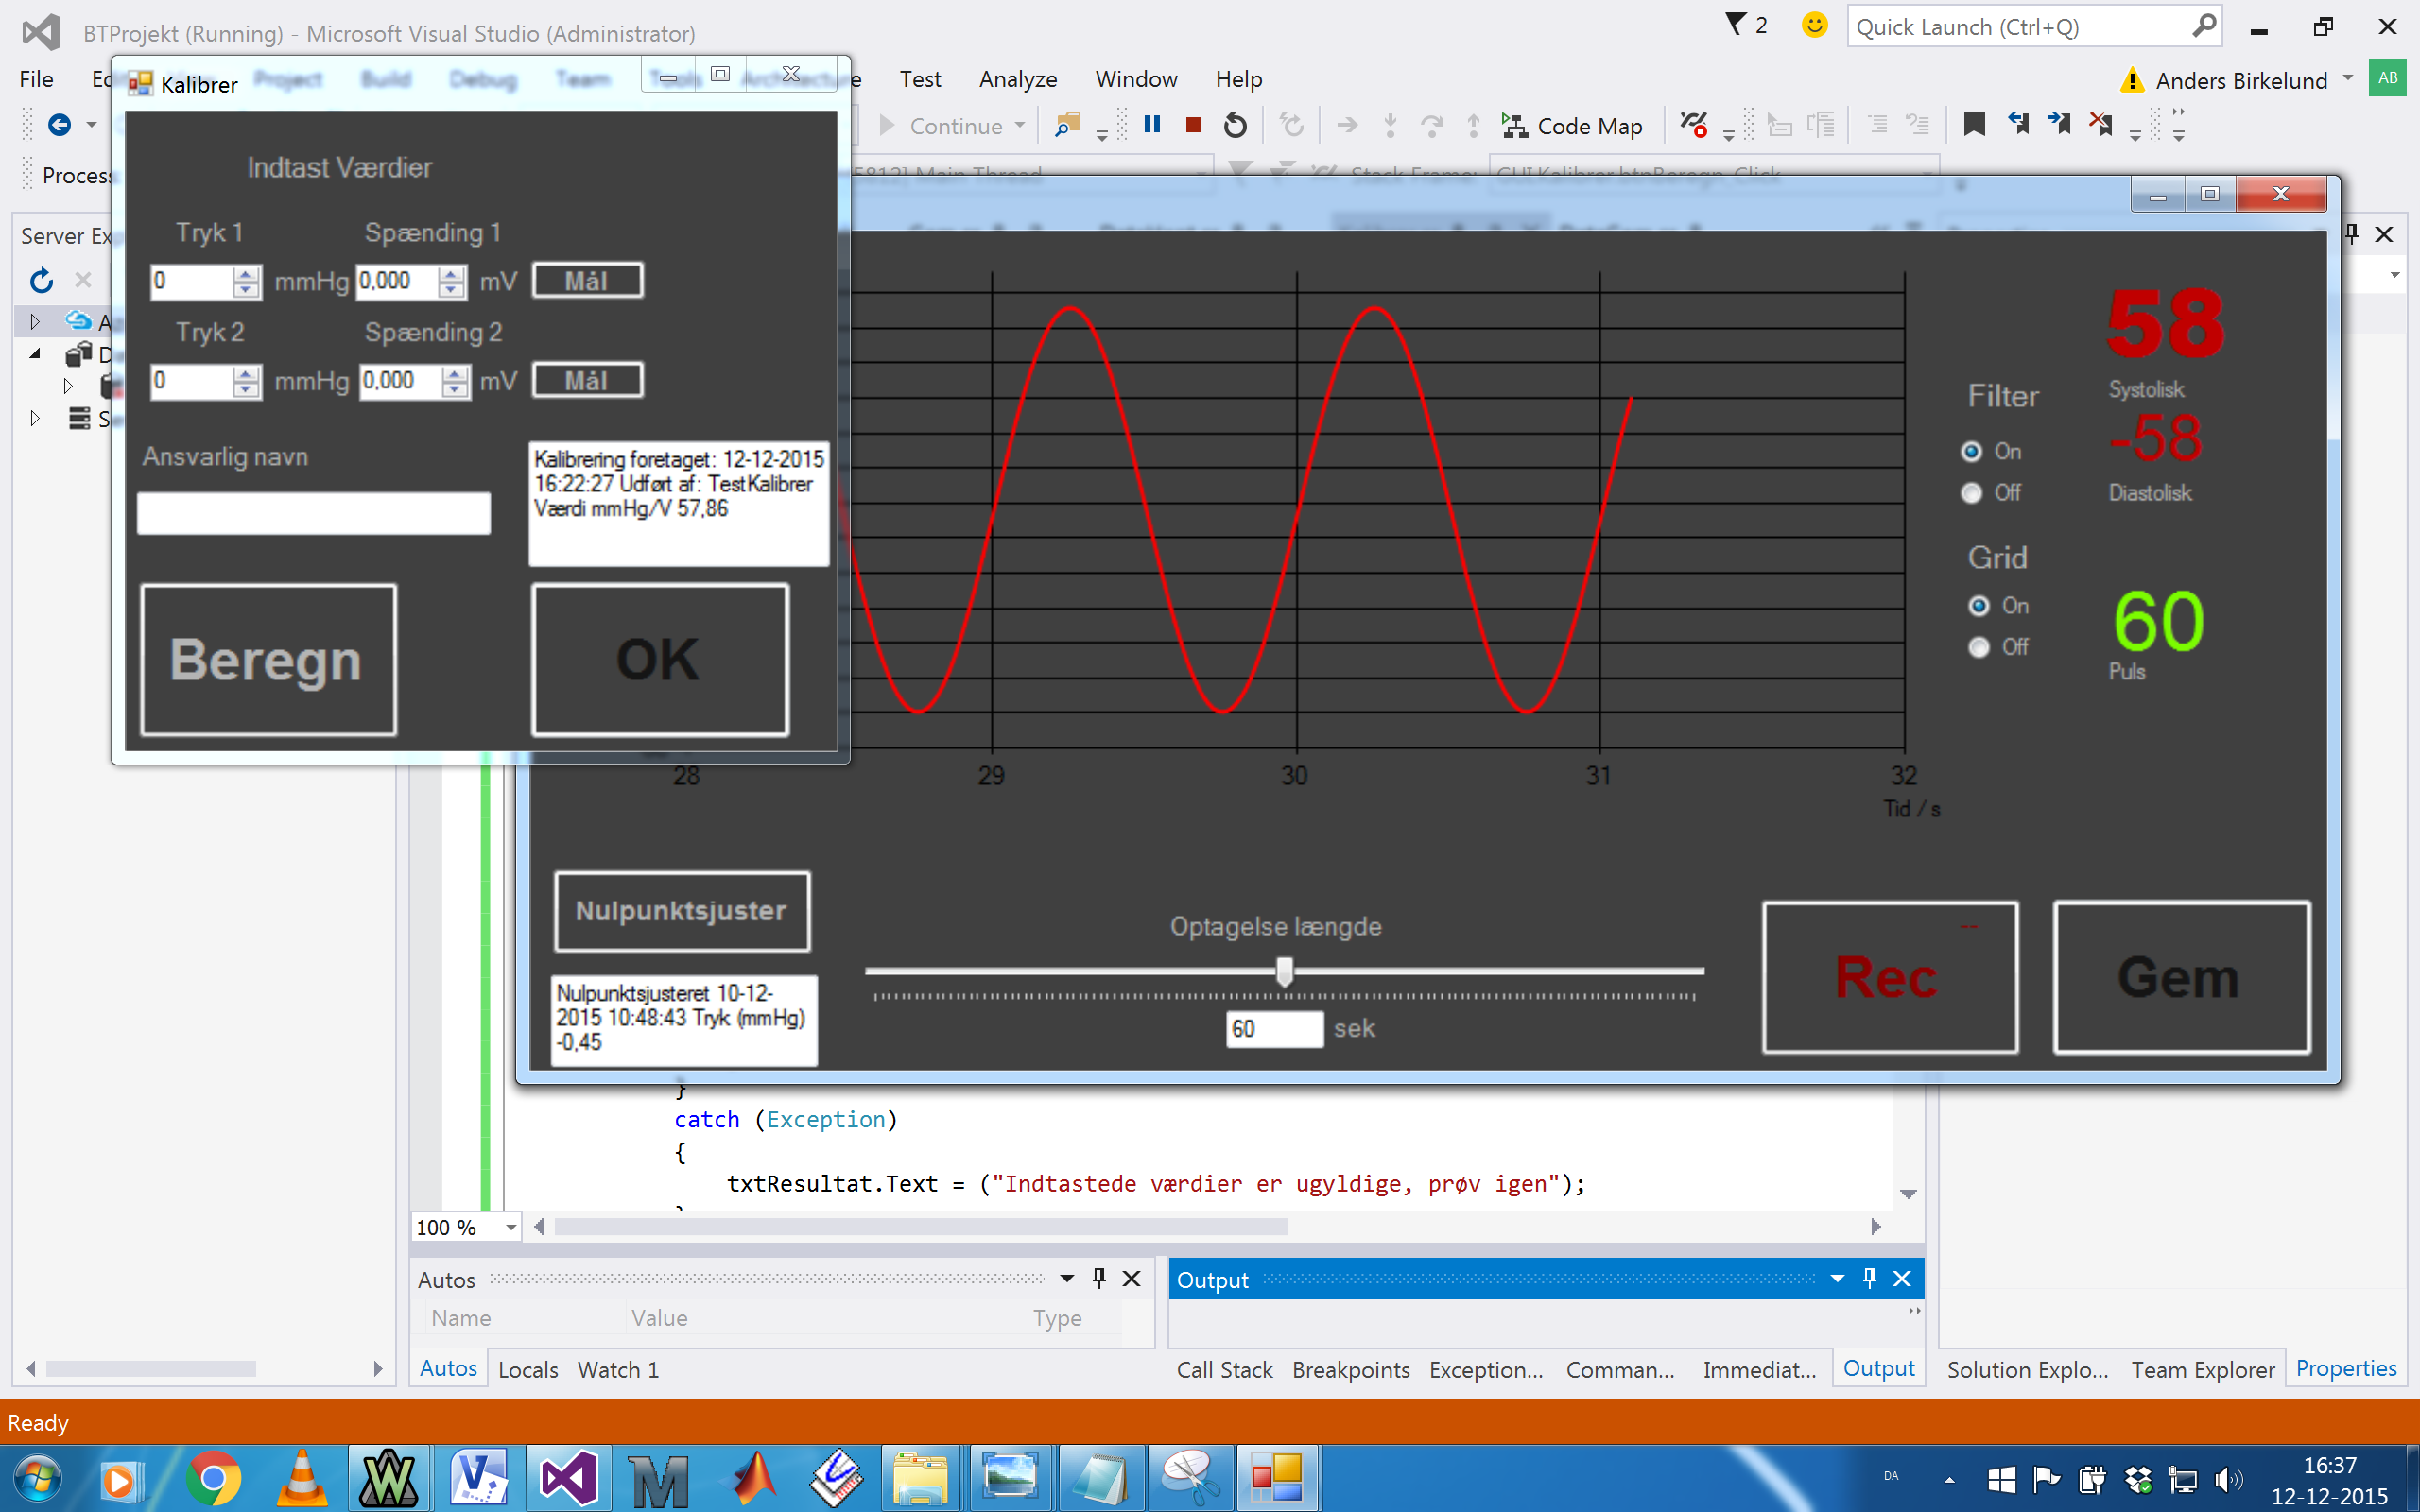
\includegraphics[width=1\textwidth]{Figurer/Test_Vis_2}
	\caption{Output på monitor-vindue}
\end{figure}




\subsection{UC3 Nulpunktsjuster}

Et DC signal på 1 V bruges til indgangssignal til DAQ.
\begin{figure}[H]
	\centering
	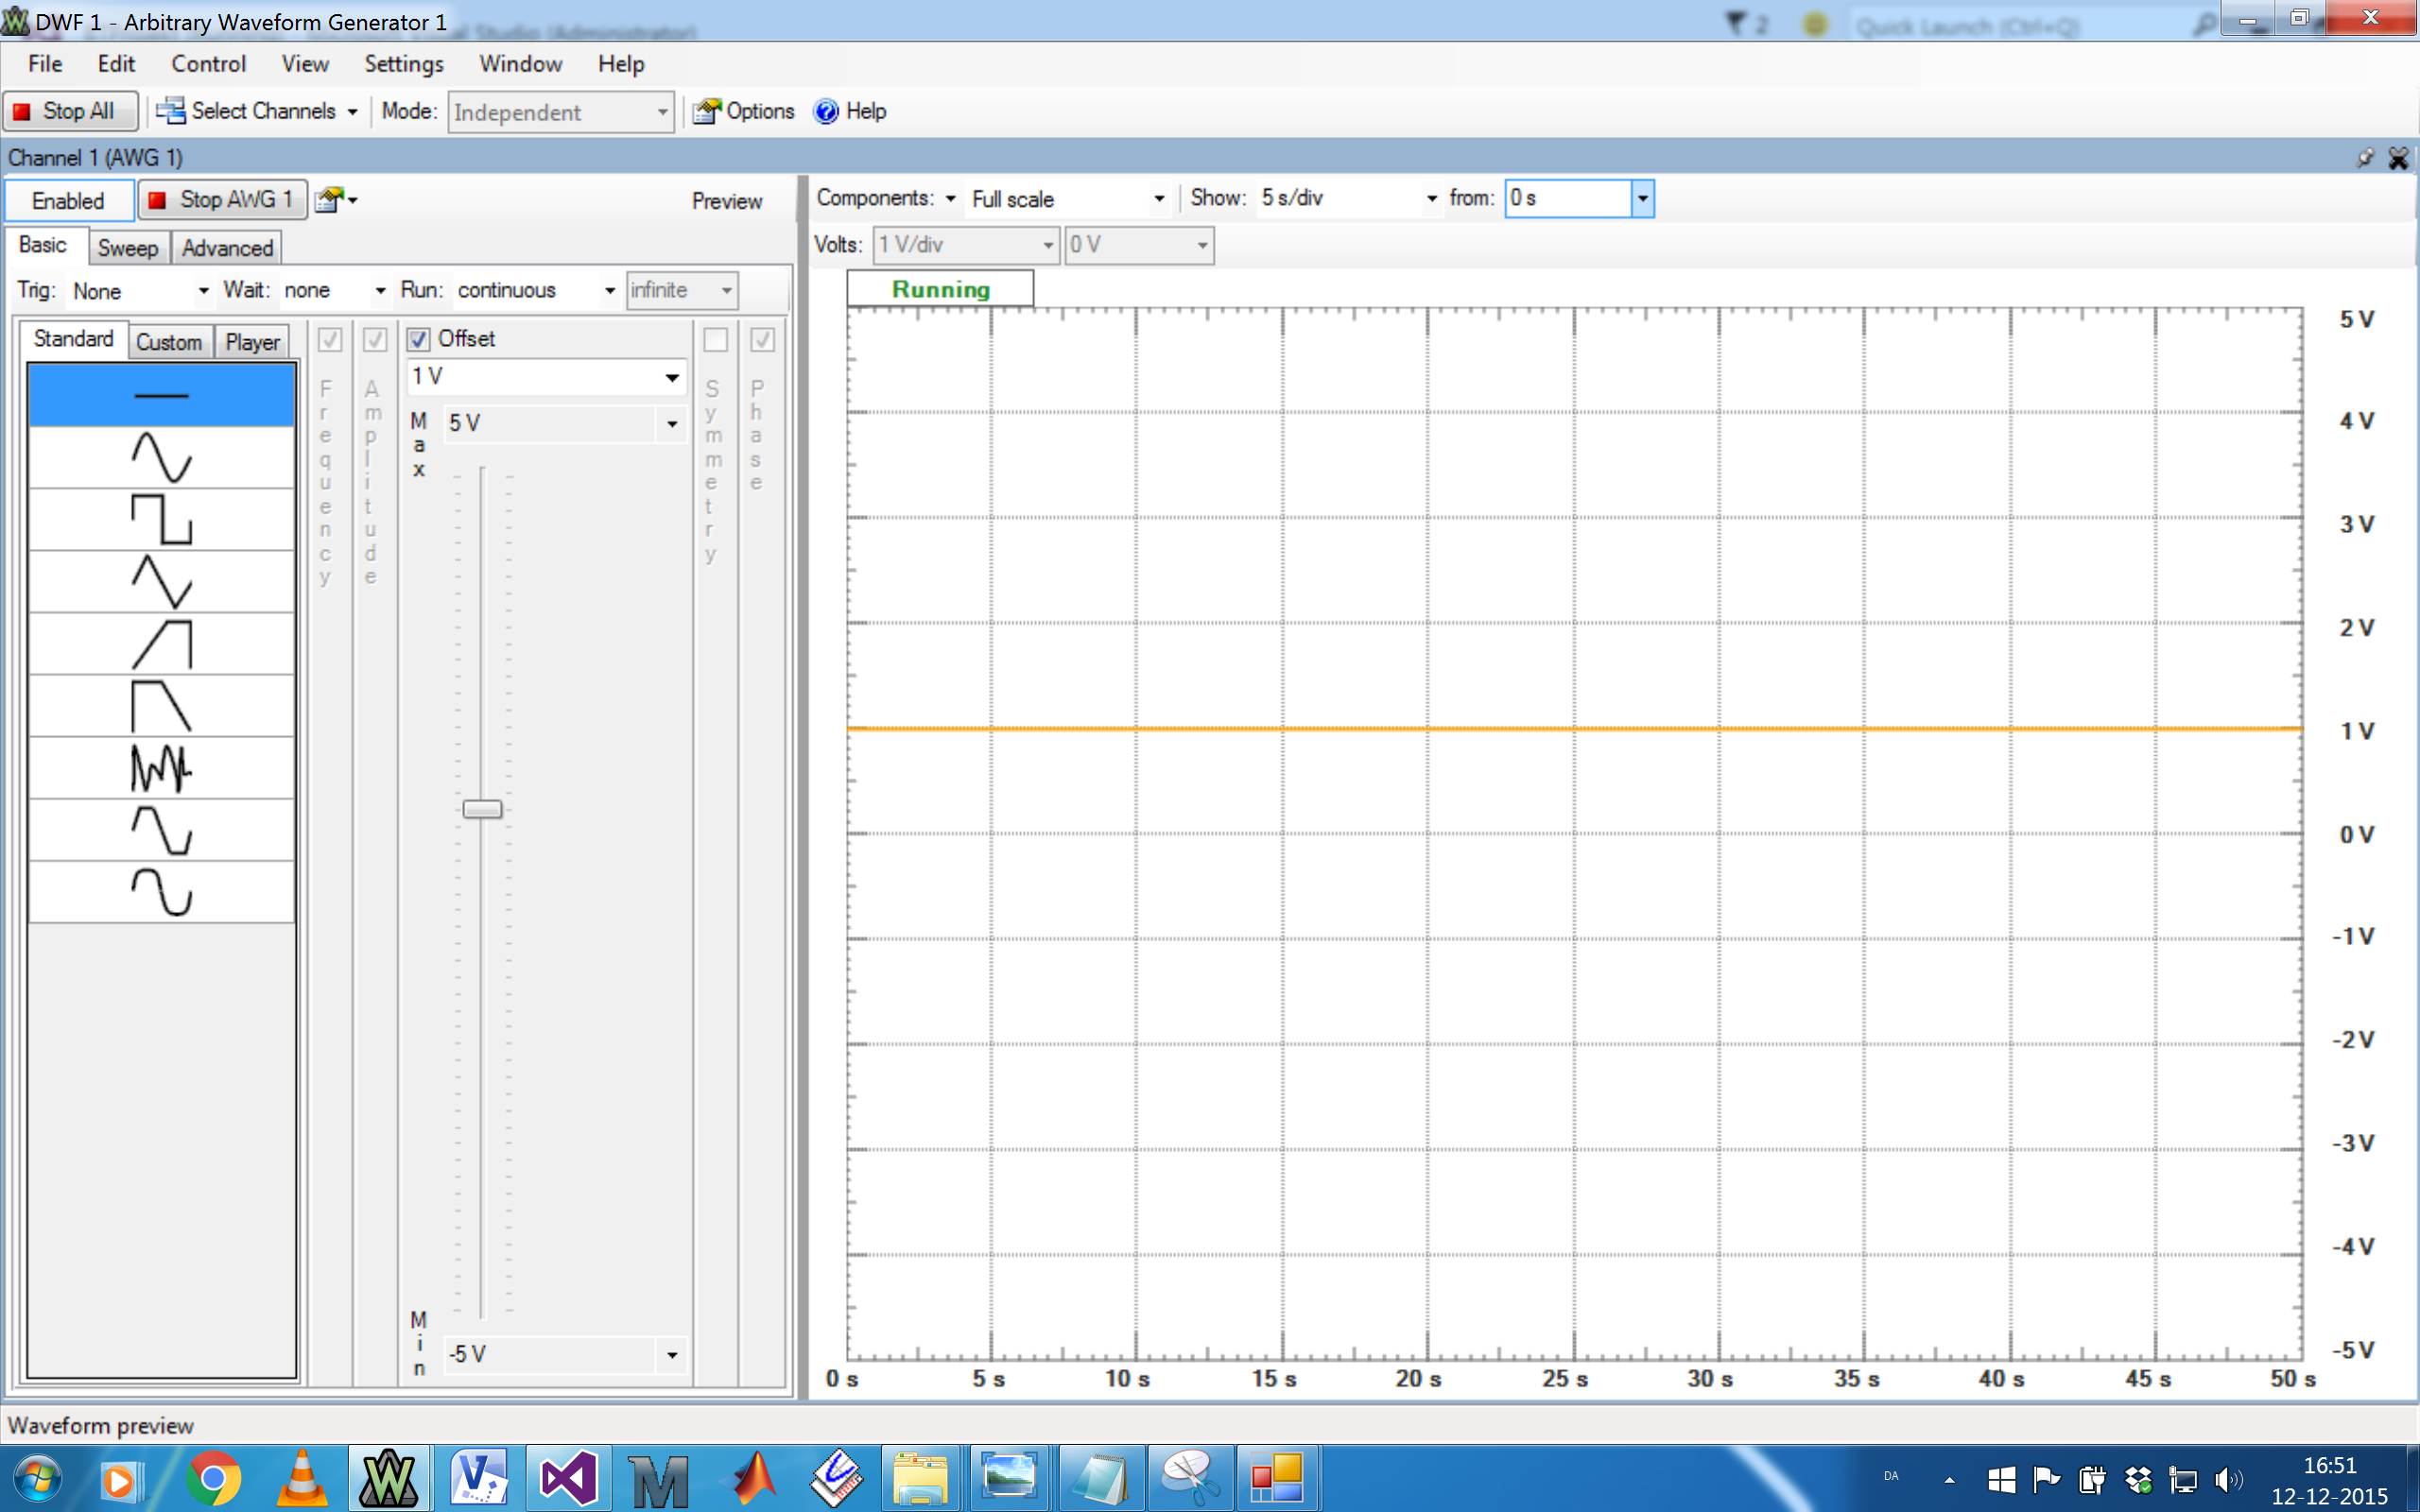
\includegraphics[width=1\textwidth]{Figurer/Test_Nul_1}
	\caption{Inputsignal til DAQ}
\end{figure}

Det ses at kalibreringskonstanten er på 57, og inputsignalet genererer det korrekte "blodtryk"
\begin{figure}[H]
	\centering
	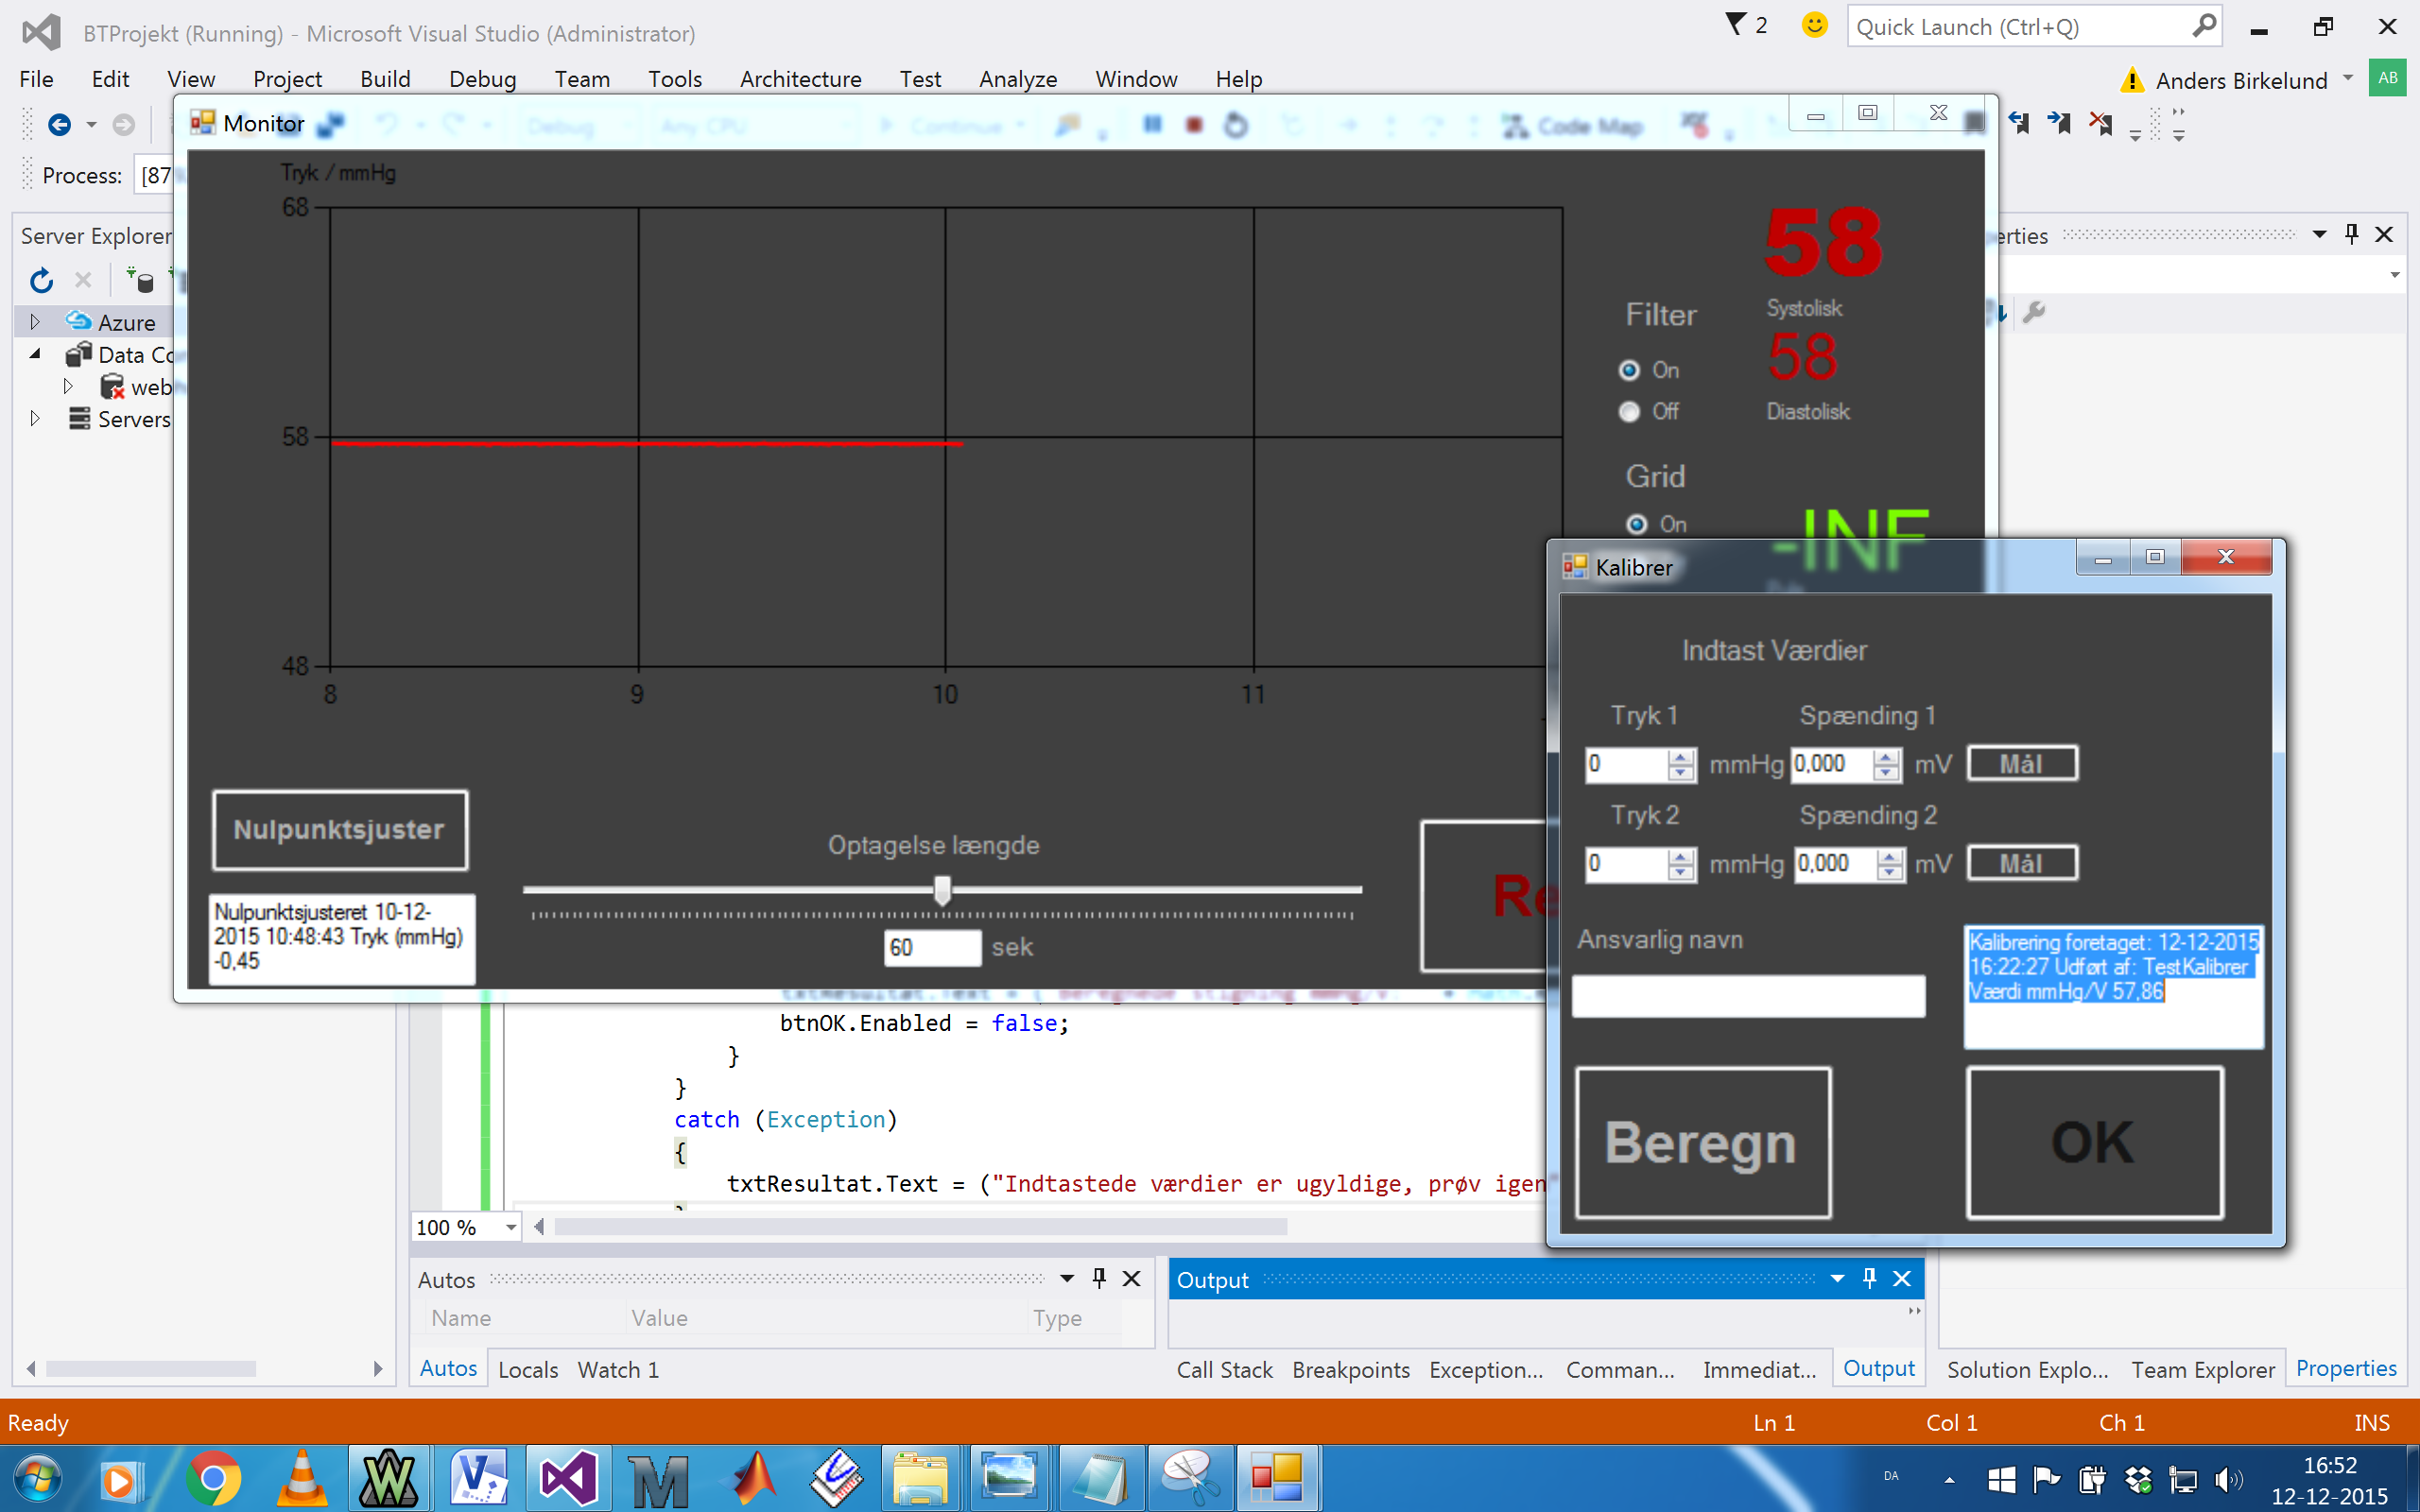
\includegraphics[width=1\textwidth]{Figurer/Test_Nul_2}
	\caption{Inputsignal til DAQ}
\end{figure}

Der trykkes på knappen "Nulpunktsjuster" og grafens værdi falder til 0. 

\begin{figure}[H]
	\centering
	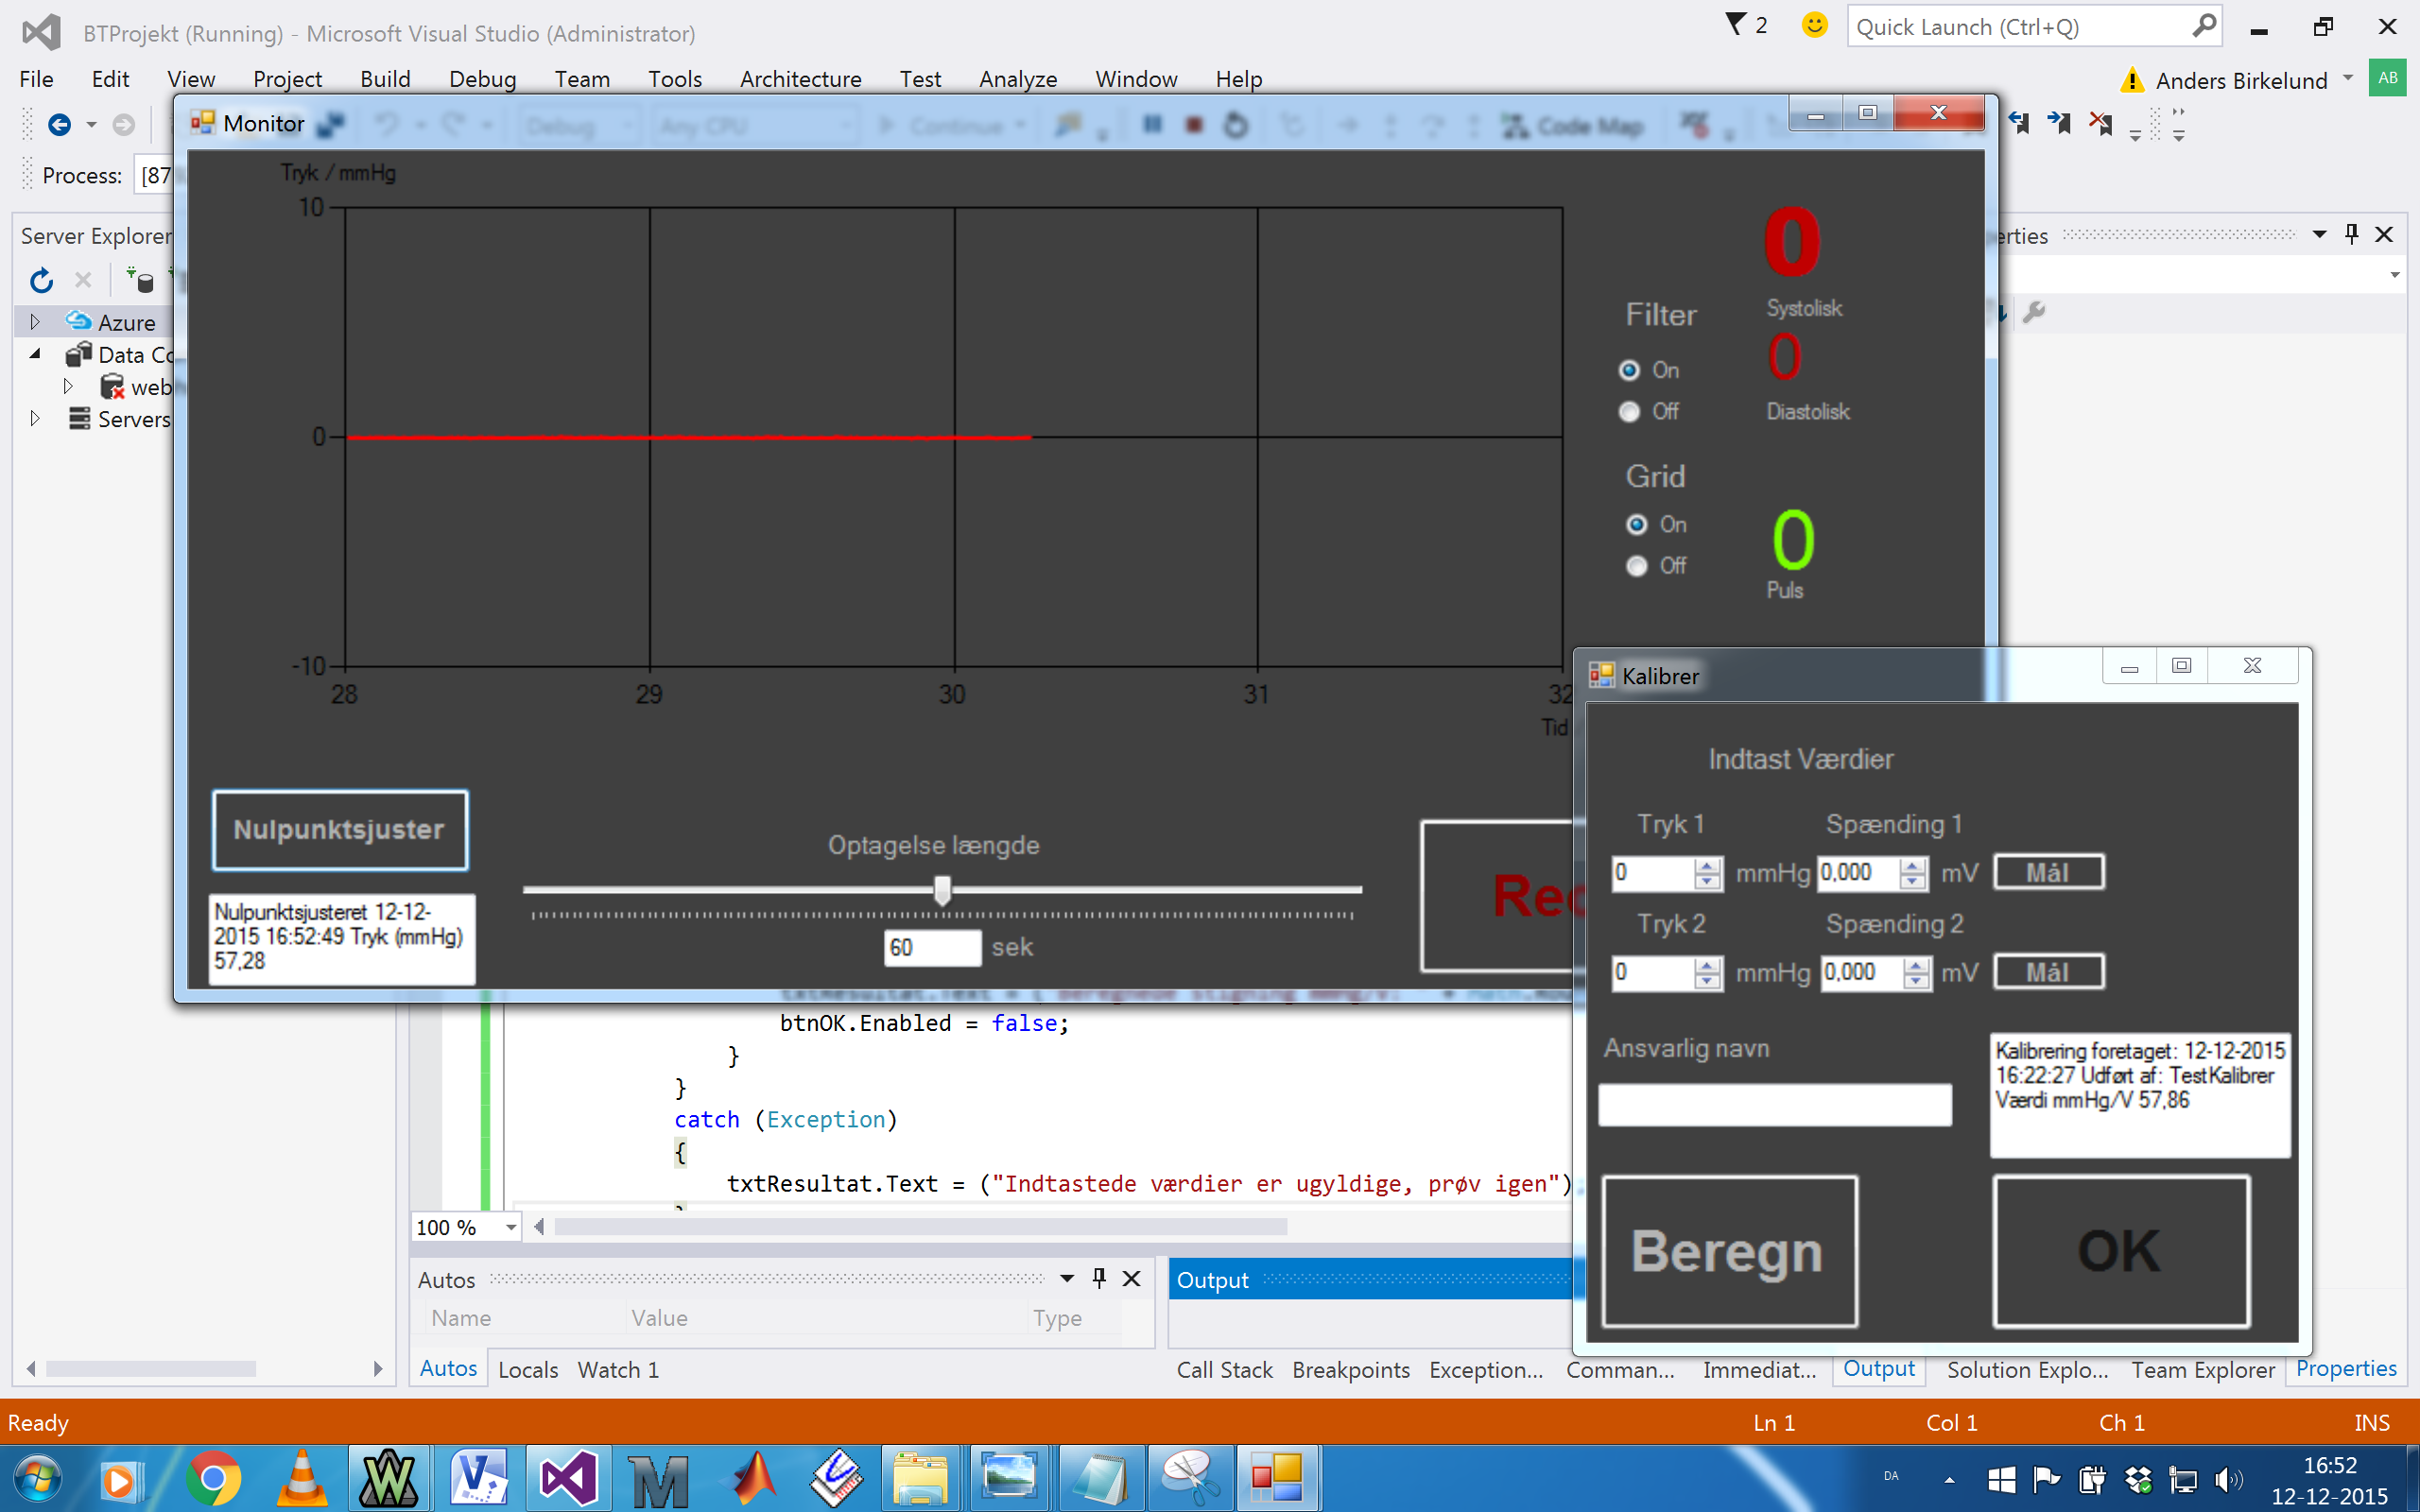
\includegraphics[width=1\textwidth]{Figurer/Test_Nul_3}
	\caption{Inputsignal til DAQ}
\end{figure}









\subsection{Filter}



Filteret er bygget op som et FIR-filter med 10 filterkoefficienter. Hver udskrevet punkt på grafen, er et gennemsnitsværdi af de foregående 10 værdier.


I denne liste indsættes en variabel, som sørger for at samples stiger med 10 pr. indsat værdi. Spændingen findes ved at tage y-værdien til den givne sample og de foregående ni værdier og beregner gennemsnittet af disse. Denne værdi indsættes i listen for vores filter, som så videre kan behandles før den udskrives i Monitor-vinduet.

